% Options for packages loaded elsewhere
\PassOptionsToPackage{unicode}{hyperref}
\PassOptionsToPackage{hyphens}{url}
%
\documentclass[
  parskip,
  oneside]{scrreprt}
\author{}
\date{\vspace{-2.5em}}

\usepackage{amsmath,amssymb}
\usepackage{lmodern}
\usepackage{iftex}
\ifPDFTeX
  \usepackage[T1]{fontenc}
  \usepackage[utf8]{inputenc}
  \usepackage{textcomp} % provide euro and other symbols
\else % if luatex or xetex
  \usepackage{unicode-math}
  \defaultfontfeatures{Scale=MatchLowercase}
  \defaultfontfeatures[\rmfamily]{Ligatures=TeX,Scale=1}
\fi
% Use upquote if available, for straight quotes in verbatim environments
\IfFileExists{upquote.sty}{\usepackage{upquote}}{}
\IfFileExists{microtype.sty}{% use microtype if available
  \usepackage[]{microtype}
  \UseMicrotypeSet[protrusion]{basicmath} % disable protrusion for tt fonts
}{}
\makeatletter
\@ifundefined{KOMAClassName}{% if non-KOMA class
  \IfFileExists{parskip.sty}{%
    \usepackage{parskip}
  }{% else
    \setlength{\parindent}{0pt}
    \setlength{\parskip}{6pt plus 2pt minus 1pt}}
}{% if KOMA class
  \KOMAoptions{parskip=half}}
\makeatother
\usepackage{xcolor}
\IfFileExists{xurl.sty}{\usepackage{xurl}}{} % add URL line breaks if available
\IfFileExists{bookmark.sty}{\usepackage{bookmark}}{\usepackage{hyperref}}
\hypersetup{
  hidelinks,
  pdfcreator={LaTeX via pandoc}}
\urlstyle{same} % disable monospaced font for URLs
\usepackage{color}
\usepackage{fancyvrb}
\newcommand{\VerbBar}{|}
\newcommand{\VERB}{\Verb[commandchars=\\\{\}]}
\DefineVerbatimEnvironment{Highlighting}{Verbatim}{commandchars=\\\{\}}
% Add ',fontsize=\small' for more characters per line
\usepackage{framed}
\definecolor{shadecolor}{RGB}{248,248,248}
\newenvironment{Shaded}{\begin{snugshade}}{\end{snugshade}}
\newcommand{\AlertTok}[1]{\textcolor[rgb]{0.94,0.16,0.16}{#1}}
\newcommand{\AnnotationTok}[1]{\textcolor[rgb]{0.56,0.35,0.01}{\textbf{\textit{#1}}}}
\newcommand{\AttributeTok}[1]{\textcolor[rgb]{0.77,0.63,0.00}{#1}}
\newcommand{\BaseNTok}[1]{\textcolor[rgb]{0.00,0.00,0.81}{#1}}
\newcommand{\BuiltInTok}[1]{#1}
\newcommand{\CharTok}[1]{\textcolor[rgb]{0.31,0.60,0.02}{#1}}
\newcommand{\CommentTok}[1]{\textcolor[rgb]{0.56,0.35,0.01}{\textit{#1}}}
\newcommand{\CommentVarTok}[1]{\textcolor[rgb]{0.56,0.35,0.01}{\textbf{\textit{#1}}}}
\newcommand{\ConstantTok}[1]{\textcolor[rgb]{0.00,0.00,0.00}{#1}}
\newcommand{\ControlFlowTok}[1]{\textcolor[rgb]{0.13,0.29,0.53}{\textbf{#1}}}
\newcommand{\DataTypeTok}[1]{\textcolor[rgb]{0.13,0.29,0.53}{#1}}
\newcommand{\DecValTok}[1]{\textcolor[rgb]{0.00,0.00,0.81}{#1}}
\newcommand{\DocumentationTok}[1]{\textcolor[rgb]{0.56,0.35,0.01}{\textbf{\textit{#1}}}}
\newcommand{\ErrorTok}[1]{\textcolor[rgb]{0.64,0.00,0.00}{\textbf{#1}}}
\newcommand{\ExtensionTok}[1]{#1}
\newcommand{\FloatTok}[1]{\textcolor[rgb]{0.00,0.00,0.81}{#1}}
\newcommand{\FunctionTok}[1]{\textcolor[rgb]{0.00,0.00,0.00}{#1}}
\newcommand{\ImportTok}[1]{#1}
\newcommand{\InformationTok}[1]{\textcolor[rgb]{0.56,0.35,0.01}{\textbf{\textit{#1}}}}
\newcommand{\KeywordTok}[1]{\textcolor[rgb]{0.13,0.29,0.53}{\textbf{#1}}}
\newcommand{\NormalTok}[1]{#1}
\newcommand{\OperatorTok}[1]{\textcolor[rgb]{0.81,0.36,0.00}{\textbf{#1}}}
\newcommand{\OtherTok}[1]{\textcolor[rgb]{0.56,0.35,0.01}{#1}}
\newcommand{\PreprocessorTok}[1]{\textcolor[rgb]{0.56,0.35,0.01}{\textit{#1}}}
\newcommand{\RegionMarkerTok}[1]{#1}
\newcommand{\SpecialCharTok}[1]{\textcolor[rgb]{0.00,0.00,0.00}{#1}}
\newcommand{\SpecialStringTok}[1]{\textcolor[rgb]{0.31,0.60,0.02}{#1}}
\newcommand{\StringTok}[1]{\textcolor[rgb]{0.31,0.60,0.02}{#1}}
\newcommand{\VariableTok}[1]{\textcolor[rgb]{0.00,0.00,0.00}{#1}}
\newcommand{\VerbatimStringTok}[1]{\textcolor[rgb]{0.31,0.60,0.02}{#1}}
\newcommand{\WarningTok}[1]{\textcolor[rgb]{0.56,0.35,0.01}{\textbf{\textit{#1}}}}
\usepackage{graphicx}
\makeatletter
\def\maxwidth{\ifdim\Gin@nat@width>\linewidth\linewidth\else\Gin@nat@width\fi}
\def\maxheight{\ifdim\Gin@nat@height>\textheight\textheight\else\Gin@nat@height\fi}
\makeatother
% Scale images if necessary, so that they will not overflow the page
% margins by default, and it is still possible to overwrite the defaults
% using explicit options in \includegraphics[width, height, ...]{}
\setkeys{Gin}{width=\maxwidth,height=\maxheight,keepaspectratio}
% Set default figure placement to htbp
\makeatletter
\def\fps@figure{htbp}
\makeatother
\setlength{\emergencystretch}{3em} % prevent overfull lines
\providecommand{\tightlist}{%
  \setlength{\itemsep}{0pt}\setlength{\parskip}{0pt}}
\setcounter{secnumdepth}{5}
\newlength{\cslhangindent}
\setlength{\cslhangindent}{1.5em}
\newlength{\csllabelwidth}
\setlength{\csllabelwidth}{3em}
\newlength{\cslentryspacingunit} % times entry-spacing
\setlength{\cslentryspacingunit}{\parskip}
\newenvironment{CSLReferences}[2] % #1 hanging-ident, #2 entry spacing
 {% don't indent paragraphs
  \setlength{\parindent}{0pt}
  % turn on hanging indent if param 1 is 1
  \ifodd #1
  \let\oldpar\par
  \def\par{\hangindent=\cslhangindent\oldpar}
  \fi
  % set entry spacing
  \setlength{\parskip}{#2\cslentryspacingunit}
 }%
 {}
\usepackage{calc}
\newcommand{\CSLBlock}[1]{#1\hfill\break}
\newcommand{\CSLLeftMargin}[1]{\parbox[t]{\csllabelwidth}{#1}}
\newcommand{\CSLRightInline}[1]{\parbox[t]{\linewidth - \csllabelwidth}{#1}\break}
\newcommand{\CSLIndent}[1]{\hspace{\cslhangindent}#1}
\usepackage[utf8]{inputenc}
\usepackage[T1]{fontenc}
\usepackage{lmodern}
\usepackage[onehalfspacing]{setspace}
\usepackage[left=2.50cm, right=2.50cm, top=2.50cm, bottom=2.50cm, bindingoffset=10mm, includehead, includefoot]{geometry}
\usepackage[headsepline]{scrlayer-scrpage}
\usepackage{url}
\usepackage[backend=biber, style=authoryear, giveninits=true, maxbibnames=99, uniquename=init, maxcitenames=2, hyperref=true, date=year]{biblatex}
\usepackage{xpatch}
\usepackage{csquotes}
\usepackage{amsmath}
\usepackage{listings}
\usepackage{booktabs}
\usepackage{longtable}
\usepackage{multirow}
\usepackage{rotating}
\usepackage{subfigure}
\usepackage{graphicx}
\usepackage{float}
\usepackage{acronym}
\usepackage{lipsum}
\usepackage{scrhack}
\emergencystretch=50pt
\clubpenalty = 10000
\widowpenalty = 10000
\displaywidowpenalty = 10000
\automark[section]{chapter}
\renewcommand*{\chaptermarkformat}{}
\renewcommand*{\sectionmarkformat}{}
\setkomafont{title}{\sffamily}
\setkomafont{disposition}{\usekomafont{title}}
\setkomafont{author}{\usekomafont{title}}
\setkomafont{date}{\usekomafont{title}}
\setkomafont{caption}{\sffamily\small}
\setkomafont{captionlabel}{\usekomafont{caption}\bfseries\small}
\setkomafont{pagehead}{\normalfont\scshape}
\ifLuaTeX
  \usepackage{selnolig}  % disable illegal ligatures
\fi

\begin{document}

\begin{titlepage}
\centering
    {\Large Ruprecht-Karls-University Heidelberg\\
        Faculty for Life Sciences\\
        Molecular Biotechnology\\}

    {\vspace{\stretch{2}}}
    {\usekomafont{title}

        {\Huge Thyorid cancer: Comparison of linar model and neuronal network (xxx)}

        {\Huge 3-Sätze-Zusammenfassung}

        {\Huge sfsf}

    }

    \vspace{\stretch{2}}
    {\Large Data Science Project SoSe 2022}

    \vspace{\stretch{2}}

    {\Large
        \begin{tabular}{rl}
            Autoren & Anna Lange, David Matuschek, Jakob Then, Maren Schneider\\
            Geburtsort & Heidelberg\\
            Abgabetermin &20.07.2022\\
        \end{tabular}
    }

    \vspace{\stretch{1}}

\end{titlepage}

\tableofcontents

\renewcommand\abstractname{\Large Acknowledgments}
\begin{abstract}
Thank You
\end{abstract}

\renewcommand\abstractname{\Large Abstract}
\begin{abstract}
Thank You
\end{abstract}

\hypertarget{introduction}{%
\chapter{Introduction}\label{introduction}}

In 2019, 230,000 humans died from cancer in Germany xxx \[[Krebsrate und
Krebs-Sterberate in Deutschland
(krebsinformationsdienst.de)](https://www.krebsinformationsdienst.de/tumorarten/grundlagen/krebsstatistiken.php)\].
To detect and fight tumors, the development of new treatment and
detection methods is essential. Therefore it is inevitable to find a
tumors mutational cause. Therefore transcriptomic profiling methods like
RNA-seq can be used.

The provided data in the following analysis originates from
transcriptomic profiling methods like RNA-seq. Transcriptomic profiling
sequences all the RNA that has been generated by transcription of a
cells DNA. The difference to sequencing of DNA is, that it only
sequences those genes, that are going to be expressed in that cell
(Alberts and Walter, 2015).

\hypertarget{hallmarks-of-cancer}{%
\section{Hallmarks of cancer}\label{hallmarks-of-cancer}}

The Hallmarks of Cancer are properties of tumors, that can be detected
in each tumor. Among others resisting cell death, inducing angiogenesis,
enabling replicative immortality, activating invasion and metastasis
evading growth suppressors were the first detected hallmarks (Hanahan
and Weinberg, 2011).

\hypertarget{histological-tumor-types}{%
\section{Histological tumor types}\label{histological-tumor-types}}

The observed tumors can be classified into different histological types.
Carcinomas contain adenocarcinomas, Squamous cell carcinoma,
transitional cell carcinoma and carcinomas in general, which include all
of the mixed carcinomas. Carciomas derive from epithelial cells.
Melanoma is a tumor of the skin, a sarcoma derives from connective or
supportive tissue cells. A glioblastoma is a tumor in the brain and
leukemia affects the blood (Alberts and Walter, 2015).

\hypertarget{rna-sequencing-xxx}{%
\section{RNA-sequencing xxx}\label{rna-sequencing-xxx}}

RNA-sequencing (RNA-seq) is performed by cleaning of RNA, fragmentation,
translation of RNA to cDNA, sequencing of cDNA and comparing with the
reference genome. The advantage of RNA-seq is that it includes
information about gene expression that is especially important in the
analysis of tumors such as epigenetic changes (e.g.~epigenetic gene
silencing) or fusion proteins (Alberts and Walter, 2015).

The results from RNA-seq used for the analysis originate from the cancer
genome atlas (TCGA).

\hypertarget{thyroid-carcinoma}{%
\section{Thyroid carcinoma}\label{thyroid-carcinoma}}

Thyroid carcinoma (THCA) incidence increased dramatically over the past
few years (Cabanillas \emph{et al.}, 2016). To enlarge the understanding
of THCA and thereby hopefully improve patients prognosis, this project
focuses on finding genes that have a significantly different expression
in THCA compared to other cancers and especially to normal
tissue.\textbackslash{} The main tasks of the thyroid gland are
synthesizing hormones and regulating body temperate and metabolism
(Tsibulnikov \emph{et al.}, 2020). A lack of thyroid hormones can cause
symptoms like headaches, nausea and depression. Most THCAs derive from
thyroid cells and thereby the thyroid gland loses their function,
resulting in a lack of thyroid hormones.\textbackslash{} Thyroid cancer
can occur in two different types, differentiated and undifferentiated
thyroid cancer. Those two types again have histological subtypes.
Papillary thyroid cancer (PTC), the most common THCA, follicular thyroid
cancer (FTC) and tall cell variant cancer (TCV) are subtypes of
differentiated thyroid cancer (DTC) while medullary and anaplastic
thyroid cancer are subtypes of undifferentiated thyroid cancer (UTC).
Prevalence of DTCs is clearly higher than of UTCs (Prete \emph{et al.},
2020).\textbackslash{} Regarding the presented DTCs, PTCs have the best
clinical prognosis (Lin, 2007), while TCV cancers have the worst
clinical outcome (Coca-Pelaz \emph{et al.}, 2020). Therefore, the
detection of the tumor type would be important and for more specific
therapy options. Even though, all thyroid cancers are treated with
thyroidectomy and radioactive iodine, the additional therapy differs for
each histological type (Kant \emph{et al.}, 2020).

\hypertarget{integrin}{%
\subsubsection{Integrin}\label{integrin}}

xxx

\hypertarget{computational-tools}{%
\section{Computational tools}\label{computational-tools}}

\hypertarget{gene-set-enrichment-analysis}{%
\subsection{Gene Set Enrichment
Analysis}\label{gene-set-enrichment-analysis}}

To analyse and compare the activity of pathways of gene expression data,
a Gene Set Enrichment Analysis (GSEA) is performed. The aim of the GSEA
is to analyse and to identify highly expressed pathways (Reimand
\emph{et al.}, 2019). For this, two conditions with replicates are
compared, so a reference of normal expression data is
needed.\textbackslash{} First, a gene list is defined. Then the
statistically enriched pathways are identified and lastly, the results
are visualized.\textbackslash{} GSEA is performed with the package
`fgsea' ref(xxx).

\hypertarget{gene-set-variation-analysis}{%
\subsection{Gene Set Variation
Analysis}\label{gene-set-variation-analysis}}

The Gene Set Variation Analysis (GSVA) is performed with the same
intention as the GSEA, so to analyse the pathway activities from gene
expression data. Like the GSEA, the approach helps to reduce noise, to
further reduce dimensions and to improve the interpretation process
(Hänzelmann \emph{et al.}, 2013). The difference to the GSEA is that
there no reference expression data is to perform the GSVA.

GSVA is performed with the package xxx.

\hypertarget{uniform-manifold-approximation-and-projection-for-dimension-reduction}{%
\subsection{Uniform Manifold Approximation and Projection for Dimension
Reduction}\label{uniform-manifold-approximation-and-projection-for-dimension-reduction}}

The Uniform manifold approximation and projection for dimension
reduction (UMAP) is a method to reduce the dimension of a
multidimensional data set. In comparison to the PCA, UMAP can reduce
dimensions where the data is not linear (Sharma \emph{et al.}, 2021).
Thereby, the high dimensional structure of the data is maintained. In
further visualization, the structure can be represented in clusters that
would not be visible using PCA. Therefore, the identification of the
clusters is a lot easier. is Thereby the UMAP keeps the overall
structure of the data set, therefore clusters are
easier.\textbackslash{} The problem of the UMAP is, that although the
overall structure is conserved, the distance between the individual
points is not proportional to the real distance in the data set. This
arises from the non-linear dimensional reduction.

UMAP is performed with the package xxx.

\hypertarget{principal-component-analysis-xxx-quelle}{%
\subsection{Principal component analysis xxx
QUELLE}\label{principal-component-analysis-xxx-quelle}}

A Principal component analysis (PCA) is used to reduce the dimension of
a given data set. The dimensions are summarized in principal components
(PCs) which do not correlate. Because the PCs summarize the dimensions,
the first PCs explain most of the variance of the data set and thereby
can be selected to explain the data. Still, one has to keep in mind,
that by reducing the dimensions, not all of the variance is explained
and some of the information is lost in the process. The ideal number of
PCs can be determined with an elbow-plot. In our analysis we use a PCA
as a foundation for the UMAP, because the UMAP can not work with
correlated dimensions. Furthermore it is used to detect the most
important pathways, which explain most of the first PCs.

In the analysis, a PCA is performed for the pan cancer analysis on the
TCGA gene expression data, to find similarities and differences in
pathway activity for each tumor type. Furthermore a PCA is performed for
the focused analysis of THCA and normal tissue.

PCA is performed with xxx.

\hypertarget{jaccard-index}{%
\subsection{Jaccard index}\label{jaccard-index}}

The Jaccard index is the intersection, divided by the union of two sets.
Therefore, it can be used to identify the similarity of the sets.

\hypertarget{pan-cancer-analysis}{%
\section{Pan Cancer Analysis}\label{pan-cancer-analysis}}

For the pan cancer analysis 3 data sets are provided. One containing
expression data of 60,000 genes in 10,000 tumor patients, another one
with clinical annotations concerning those patients and one with
hallmark pathways and their included genes. In the following analysis
this data is cleaned by removing NAs, biotype filtering and low-variance
filtering. After that a descriptive analysis is performed. Those two
steps lead to the actual analysis, a gene set variation analysis to
detect significantly altered pathways compared to the other pathways in
tumor tissue. In the end a linear regression analysis is performed to
predict pathway activity based on other pathways??? xxx Furthermore a
neuronal network is built to improve prediction.

\hypertarget{focused-analysis-on-thca-patients}{%
\section{Focused analysis on THCA
patients}\label{focused-analysis-on-thca-patients}}

Furthermore a analysis of THCA patients is performed. For this analysis
a data set containing the gene expression of 60 patients in tumor an
normal tissue and their clinical annotations. First the data is cleaned
and described like the pan cancer data, to prepare the data for the gene
set variation analysis, which is also performed for the THCA data in the
bigger pan cancer data set, to confirm results from the smaller data
set. In this analysis a linear regression analysis is performed to
predict the activity of thyroxine biosynthesis. The results are also
improved with a neuronal network.

\hypertarget{linear-regression-analysis}{%
\section{Linear regression analysis}\label{linear-regression-analysis}}

A linear regression analysis is performed to predict the activity of xxx
based on the activity of the other pathways.

Firstly, the correlation of the pathways for predicting is checked, only
pathways with a low correlation were kept. In the next step, the
variance is checked, 80\% of the genes with low variance were omitted.

For the regression analysis only 20\% of the pathways were used, to only
use significant pathways.

The regression analysis was tested by

\hypertarget{neural-network}{%
\subsection{Neural network}\label{neural-network}}

Implementing a neural network was performed with the package neuralnet.

In general, a deep learning network consists of a input layer, multiple
hidden layers and an output layer. Each one consisting of various
neurons. The input layer contains as much neurons as input numbers are
given for each sample. The output layer contains as much neurons as
possible outputs. The number of neurons in each hidden layer and the
number of hidden layers vary and will be determined for the best
results.

Based on the input numbers in the input layer, the number of each neuron
of the next layer is determined, based a linear regression model
composed of the input data, weights, and bias.

\[
\sum_{i=1} ^{n} w_i x_i + bias
\]

n is the number of input neurons and \emph{w} the weight.

To obtain numbers in the range of 0 and 1, a min max scaling is
performed on the input data. Furthermore, the optimal number of neurons
per layer and the best random weights and biases for the first sample
must be determined, because some weights and biases may result in
finding a local, but not global minimum of the cost function.

After determining the random weights and bias, which resulted in a
random output for the first sample, the cost function is calculated. To
minimize the cost, resilient backpropagation with weight backtracking is
used. Therefore, the gradient function of the cost function is
determined. In resilient backpropagation, only the sign of the derivate
is used, to avoid harmful effects of its magnitude. For minimizing the
cost function, the ideal weights and biases are determined, based on the
input and the expected output. (Theoretisch kann man hier ja noch
schreiben, dass nicht nur das Erreichen des Minimums, sondern auch die
Geschwindigkeit für das Erreichen des Minimums relevant sind).

For the next samples those steps are repeated to reach the minimum of
the cost function.

\[
Cost function = \frac {1}{2m} \sum_{i=1} ^{m} (x - y)^2
\]

\emph{m} is the number of samples, \emph{y} the output and \emph{x} the
expected output.

Quelle für das ganze: (@inproceedings\{Riedmiller1994RpropD,

~ title=\{Rprop - Description and Implementation Details\},

~ author=\{Martin A. Riedmiller\},

~ year=\{1994\}

\})
\href{https://www.semanticscholar.org/paper/Rprop-Description-and-Implementation-Details-Riedmiller/a8815421205d3a8938d78db974db1d4f3584ffb6}{Rprop
- Description and Implementation Details \textbar{} Semantic Scholar}
xxx

\hypertarget{material-and-methods}{%
\chapter{Material and Methods}\label{material-and-methods}}

In the following, two analyses are performed: a pan cancer analysis and
a focused analysis about THCA.

\hypertarget{our-data-sets}{%
\section{Our data sets}\label{our-data-sets}}

For the analysis four data sets were provided.

The first data set is a Gene expression data frame. The Gene expression
data frame contains 60,000 genes and and their expression in 10,000
patients. It is derived from The Cancer Genome Atlas (TCGA). The
expression of the genes was obtained by RNA-seq.

The second data frame contains 37 clinical annotations like Tumor type,
age, gender, etc. for each of the 10,000 patients from the Gene
expression data frame.

The third object is a list that contains five lists for the focused
analysis, one list for each tumor type (BRCA, KIRC, LUAD, PRAD, THCA).
For the focused analysis, the THCA data (only DTC) was used. The THCA
data contains 3 data frames, each one with information about the same 60
patients. The first data is a gene expression matrix from THCA tissue,
the second data contains the gene expression from normal tissue and the
third data frame contains the clinical annotations like age and gender.
Gene expression data was obtained by RNA-seq.

The fourth object contains 46 pathways involved in phenotypes partly
included in the hallmarks of cancer and the genes involved in those
pathways.

SIND DIE DATEN NORMALISIERT --\textgreater{} Normalisiert glaub ich
(Anna) ODER ALS COUNTS?

\hypertarget{metabolic-pathway-selection}{%
\section{Metabolic pathway
selection}\label{metabolic-pathway-selection}}

From the Molecular Signature Database (MSigDB) \cite{xxx} metabolic
pathways were selected. First, they were compared to the given
Hallmark-Pathways in order to select pathways that differ to the
Hallmark-Pathways. The goal was to identify more pathways, that are
important for the development of cancer. Therefore it was important that
as many genes from the selected pathways as possible are also included
in the provided Hallmark pathways. To identify the relevant pathways,
the intersection of genes was calculated and the genes with an
intersection of at least 99\% were maintained for further analysis.

xxx??????????????????????

To avoid duplicates in between the metabolic pathways and between the
Hallmark pathways and the metabolic pathways, the pathways were checked
for duplicates with the Jaccard index. Pathways with a sum of Jaccard
indices beyond the 1-sigma range were discarded.

\hypertarget{preprocessing}{%
\section{Preprocessing}\label{preprocessing}}

\hypertarget{deleting-not-available-values-nas}{%
\subsection{Deleting Not Available Values
(NA's)}\label{deleting-not-available-values-nas}}

Deleting of NA's was done with the R-function na.omit(x).

\hypertarget{low-variance-filtering}{%
\subsection{Low-Variance Filtering}\label{low-variance-filtering}}

Low variance filtering is performed to delete genes with a low variance
in gene expression from the data set. It is performed to delete genes
that are expressed the same in all cancer types (pancancer analysis) or
the same in normal cells. To calculate the variance of the gene
expression of a gene, the r-function var(x) is used and genes with a
lower variance than a certain threshold value are
removed.\textbackslash{} For the focused analysis the variance of the
gene expression for each gene in tumor tissue was calculated. Genes with
a variance beneath a certain threshold were deleted in the data sets of
tumor and normal tissue.

\hypertarget{biotype-filtering}{%
\subsection{Biotype Filtering}\label{biotype-filtering}}

The biotype filtering was conducted for the pancancer data and the
focussed analysis data. The biotype of each gene was determined (protein
coding, RNA,\ldots) and compared with the biotypes of pathways. To allow
an appropriate comparison of the expression data and further reduce the
data, only biotypes were kept that are available in the pathways. The
biotype can be determined with the R-function checkbiotypes(x) from the
package biomaRt (Durinck \emph{et al.}, 2005).

\hypertarget{selection-of-metabolic-pathways}{%
\subsubsection{Selection of metabolic
pathways}\label{selection-of-metabolic-pathways}}

(da eine hohe jaccard summe eine hohe überschneidung mit anderen
pathways bedeutet. In einer heatmap sind hohe Jacccard indices weiß bis
rot gefährbt. Ein niedriger Jaccard index ist blau gefärbt.)

To test for duplicate pathways in the selected metabolic pathways
compared to the hallmark pathways and the compared tp the metabolic
pathways themselves, the Jaccard index between to pathways were
calculated.\textbackslash{} There were a few duplicates between the
metabolic and Hallmark pathways. Those metabolic pathways with a high
Jaccard index were discarded. The success of the cleaning was checked by
again calculating the Jaccard index between the metabolic and the
hallmark pathways. The values of the Jaccard index were then illustrated
in a heatmap \ref{xxxfigure heatmap}. It can be assumed, that the
selection of relevant pathways was successful because the pathways
differ between each other. The number of metabolic pathways could be
reduced from xxx to 600.

\hypertarget{descriptive-analysis}{%
\section{Descriptive analysis}\label{descriptive-analysis}}

\hypertarget{mean-variance-plot}{%
\subsection{Mean-variance plot}\label{mean-variance-plot}}

In a mean-variance plot the variance is plotted over the mean of
expression values of the single genes across all patients. Thus, the
variance and mean were calculated by the R-functions var(x) and mean(x).
This is done to determine genes, which differ a lot in their expression
levels across all patients. The plot is created with the package
\ref{ggplot2} xxx.

\hypertarget{violin-plot}{%
\subsection{Violin plot}\label{violin-plot}}

To check the distribution of a data set and compare it with other data
sets violin plots are used. Based on how similar the violin plots are,
it can be implied that the data is normalized. Violin plots are tilted
and mirrored density plots of gene expression values. The y-axis shows
the gene expression value and the x-axis shows the amount of genes with
a certain gene expression value.

\hypertarget{jaccard-index-1}{%
\subsection{Jaccard-Index}\label{jaccard-index-1}}

The Jaccard-Index is a method to describe the similarity between two
quantities. It is computed via dividing the union by the intersection.
This is used to determine the degree in which metabolic pathways are
similar to each other.

\hypertarget{volcano-plot}{%
\subsection{Volcano plot}\label{volcano-plot}}

A volcano plot is used to identify significantly differentially
expressed genes. This is done to determine genes or pathways, which are
up- or down- regulated in tumor tissue vs.~normal tissue. The mean of
each gene is calculated for normal and THCA tissue and used for the
calculation of the Log2-Foldchange (Log2FC) in the following way, since
the provided expression data is already log2 data:

\[
log2FC = mean(normal tissue) - mean(tumor tissue)
\] In the next step, a two-sided t-test was performed to determine the
significance of a difference in expression.

To avoid the accumulation of type 1 errors, a bonferroni correction was
performed. n is the number of genes in the cleaned data set for focused
analysis:

\[
\alpha = \frac{0.025}{n}
\]

In the volcano plot the -log10 of the calculated p values is plotted
against die Log2FC. Genes with a a lower p-value than the corrected
alpha-value are significantly differently expressed. If the Log2FC is
additionally higher than 0.1, the genes are significantly over expressed
in tumor tissue, if the Log2FC is higher lower than -0.1, the genes are
significantly under expressed in tumor tissue.

\hypertarget{data-reduction-and-pathway-activities}{%
\section{Data Reduction and Pathway
Activities}\label{data-reduction-and-pathway-activities}}

\hypertarget{pca}{%
\subsection{PCA}\label{pca}}

The package xxx is used to perform the PCA. Therefore the data obtained
from the GSEA was used. After performing the PCA, the results were
plotted to visualize the different clusters.

The PCA was performed for pathway and gene activity. For analysis of the
gen activity the package xxx was used. Dazu wurde noch analysiert, wie
die Pathways auf die PCs verteilt sind.

\hypertarget{umap}{%
\subsection{UMAP}\label{umap}}

Like PCA, UMAP is a technique to reduce dimensions and to understand and
visualize high dimensional data sets. Compared to PCA, UMAP better
preserves the global structure and is much faster than other comparable
techniques (for example t-SNE \cite{xxx}). The algorithm starts by
setting up a high-dimensional graph representation of the data. From
each data point, a radius is extended and when two radii come into
contact the points are connected. The radius is chosen individually for
each point based on the distance to the nearest neighbor. The algorithm
does not stop before every point is not connected at least to its
closest neighbor. The resulting clustered high-dimensional graph is then
optimized for a visualization in low-dimensions. Using this technique,
the pan-cancer data is visualized.

\hypertarget{gsea}{%
\subsection{GSEA}\label{gsea}}

The GSEA is used to identify enriched pathways in tumor tissue. Next to
the tumor tissue data, the THCA data includes also a normal tissue gene
expression data frame which is used as a reference for activity
comparison.

First, the log2FC is calculated for every gene of each each patient and
is then ranked in a vector. This vector begins with the highest log2FC
and ends with the lowest. A high log2FC implies that the this gene is
higher expressed in tumor tissue compared to normal tissue in this
particular patient.

Using the ranked log2FC vectors, the activity of each pathway for the
patient is calculated. By iterating over every gene of the ranked
vector, it was checked if it lies or does not lie in a particular
pathway. If a gene lies in the pathway, the log2FC value is summed up to
a running sum. If the gene does not lie in the pathway, the log2FC value
is subtracted from the running sum. Therefore, when a pathway is highly
expressed compared to normal tissue, the the running sum scores a high
value in the beginning and decreases to the end of the iteration. This
results in a cumulative function that has a peak at a certain place. At
this index of the ranked vector, the expression value of the
corresponding gene is taken as the enrichment score of the analysed
pathway and the patient belonging to the used vector. This process is
then repeated for each pathway and each patient.

\hypertarget{gsva}{%
\subsection{GSVA}\label{gsva}}

Next to the GSEA, the GSVA is an approach to identify the pathway
activities from gene expression data. Differently to the GSEA, it does
not need a reference data frame to compare to.\textbackslash{} Hence,
there was no expression data provided for comparison in the TCGA
analysis, GSVA was used. There are various solutions to perform GSVA,
one of them is performed by Hänzelmann et al xxx by following those five
steps.\textbackslash{} For performing a GSVA, firstly the cumulative
density distribution of a gene over all samples is estimated. Then the
expression statistic of a gene in a sample based on the cumulative
density distribution is calculated to bring all of the expression values
to the same level. The third step is to rank the genes based on the
expression statistic and to normalize the ranks with z-transformation.
The last step is to compute the enrichment score based on the obtained
ranked list. Therefore the Kolmogorov-Smirnov-like rank statistic is
calculated for each gene set. That is used to calculate the enrichment
score for each pathway in each patient, which is shown a heatmap.
(Hänzelmann, Castelo, and Guinney 2013) xxx Hänzelmann, Sonja, Robert
Castelo, and Justin Guinney. 2013. ``GSVA: Gene Set Variation Analysis
for Microarray and Rna-Seq Data.'' Journal Article. BMC Bioinformatics
14 (1): 7. \url{https://doi.org/10.1186/1471-2105-14-7.}

\hypertarget{figure-x}{%
\subsection{Figure X}\label{figure-x}}

To identify pathways with the highest p-Value, obtained from GSVA and
t-testing, a figure x is generated.

For generating figure x, the data from generating a volcano plot is used
to identify the pathways, that are significantly over- or underexpressed
based on the p-value. Pathways with a p-value smaller than 0.025 and a
log2FC bigger than zero are significantly overexpressed, if the log2FC
is smaller than zero, the pathways are significantly underexpressed. In
the next step, the pathways are ranked based on their p-value and the
-log10(p-value) of each pathways is plotted against its rank. One plot
is generated for overexpressed pathways and the other one for under
expressed pathways.

\hypertarget{linear-regression}{%
\subsection{Linear Regression}\label{linear-regression}}

\hypertarget{neuronal-network}{%
\subsection{Neuronal Network}\label{neuronal-network}}

A neural network was used to predict the activity of
REACTOME\_INTERLEUKIN\_36\_PATHWAY based on the activity of other
pathways. Therefore, the network was trained with the pathway activity
of 45 xxx patients from the THCA data for focused analysis. The other 15
patients were used to validate the network, obtaining a mean squared
error (MSE) value, to evaluate the precision of the network.

For identification of the best initial conditions, 25 different networks
are generated, each one with 2 hidden layers and different combinations
of neurons per layer. For each combination the MSE is calculated and the
3 combinations with the lowest MSE are selected for selection of the
best initial conditions regarding the weights and biases. For each of
the 3 networks 100 random initial conditions are tested, resulting in
one network with the lowest MSE.

Packages Tabelle einfügen! --\textgreater{} sorry: habe leider die zeile
gelöscht, hoffe du weißt noch, was du gemacht hast :(

\hypertarget{results}{%
\chapter{Results}\label{results}}

\hypertarget{preprocessing-1}{%
\section{Preprocessing}\label{preprocessing-1}}

\hypertarget{data-cleaning}{%
\subsection{Data cleaning}\label{data-cleaning}}

All dataframes were checked for NAs, which were subsequently deleted.
Genes with a variance lower than 0.1 were removed to reduce
dimensionality, as they contribute very little to the overall variance
of the data set and are most likely house-keeping genes. Doing so, the
number of genes in the pan-caner data set was reduced from 60,000 to
approximately 19,000 genes.

The low-variance filtering of the THCA data set was done in a similar
way. Genes with a lower variance than 0.06 were deleted in the tumor
tissue and the normal tissue data. This resulted in a reduction from
approximately 20,000 genes to 15,000 genes in both data frames.

\hypertarget{biotype-filtering-1}{%
\subsection{Biotype filtering}\label{biotype-filtering-1}}

To reduce dimensionality further, we determined biotype of the hallmark
pathway genes, which was almost exclusively protein coding. To match
this, only protein coding pathways were kept in all expression data sets
for further analysis.

\hypertarget{pathway-selection}{%
\subsection{Pathway selection}\label{pathway-selection}}

The pathways from the MSigDB database were first aligned with the genes
in our expression data. Only pathways with a coverage of over 99\% were
kept. To avoid biases during enrichment analysis jaccard indices between
hallmark pathways and MSigDB pathways were computed and pathways with a
high similarity were removed.

\hypertarget{descriptive-analysis-1}{%
\section{Descriptive analysis}\label{descriptive-analysis-1}}

\hypertarget{mean-variance-plot-of-tcga-expression-data-shows-highly-variant-genes}{%
\subsection{Mean-variance plot of TCGA expression data shows highly
variant
genes}\label{mean-variance-plot-of-tcga-expression-data-shows-highly-variant-genes}}

To determine the genes from the TCGA expression data with a high
variance, the variance was plotted over the mean (Figure
@ref(fig:showmeanvariance)). Additionally those genes with a variance
higher than 33 were labeled with their EnsembleID. The distribution of
genes in this plot shows that the highly variant genes are around a log2
mean expression level of 0. The plot also shows, that very few genes are
at a low mean expression level or at a very high mean expression level.
Most genes are expressed across all patients at a log2 mean expression
level of approximately 0. With this plot we were able to determine which
genes differ significantly in their expression level across all cancer
patients.

\begin{figure}

{\centering 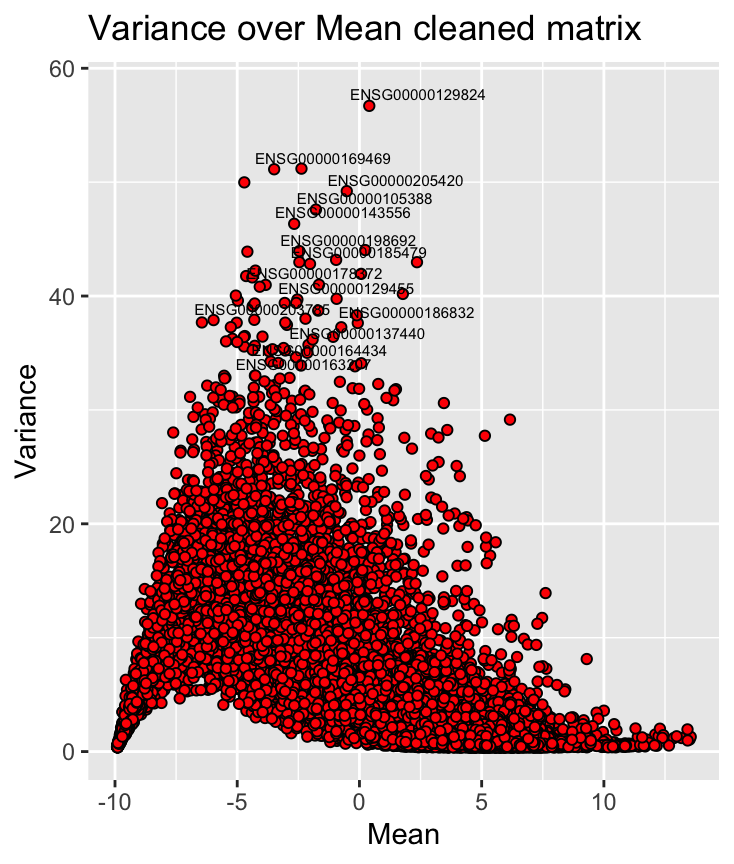
\includegraphics[width=0.3\linewidth]{figures/Variance_over mean_cleaned_matrix} 

}

\caption{Mean-variance plot of cleaned TCGA expression data. Y-axis shows variance of a genes expression, x-axis shows mean of a genes expression}\label{fig:showmeanvariance}
\end{figure}

\hypertarget{significantly-up--and-down-regulated-genes-in-thca-obtained-from-volcano-plots}{%
\subsection{Significantly up- and down regulated genes in THCA obtained
from volcano
plots}\label{significantly-up--and-down-regulated-genes-in-thca-obtained-from-volcano-plots}}

To determine those genes that are up- or down-regulated in THCA, the
expression data from tumor tissue was compared to the data from normal
tissue by mean log2 fold change. Associated p-Values were comuted with a
Wilcoxon rank sum test. (Figure @ref(fig:showvolcanoplot)). The
significance level adjusted to 1.755e-06 with a Bonferrioni adjustment.
(!!!!! WICHTIG Welche sind up-regulated, welche down-regulated???)xxx

\begin{figure}

{\centering 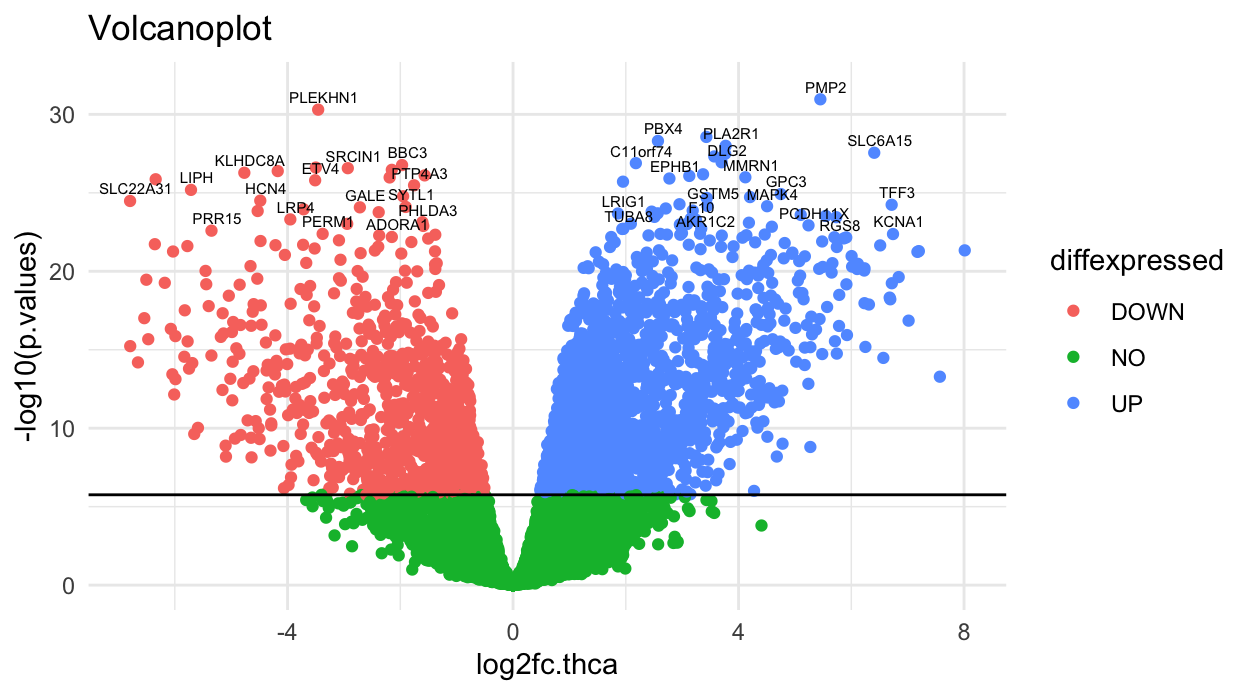
\includegraphics[width=0.3\linewidth]{figures/Volcanoplot} 

}

\caption{Volcano plot of THCA expression data}\label{fig:showvolcanoplot}
\end{figure}

\hypertarget{pan-cancer-analysis-1}{%
\section{Pan cancer analysis}\label{pan-cancer-analysis-1}}

\hypertarget{gsva-of-tcga-expression-data-reveals-four-clusters-of-cancer-types}{%
\subsection{GSVA of TCGA expression data reveals four clusters of cancer
types}\label{gsva-of-tcga-expression-data-reveals-four-clusters-of-cancer-types}}

To find general clusters a heatmap with the mean expression of each gene
in each tumor type was generated and clustered hierarchically. Figure
@ref(fig:meanexp)

The tumor types were clustered based on their mean pathway activity and
formed four clusters correlating with their histological type. The first
cluster contains mainly adenocarcinamas, while the second one contains
predominately glioblastomas. Leukemias are only found in the third
cluster and the last cluster is enriched with sarcomas and carcinomas.
Melanomas appear in the second and fourth cluster.

Furthermore, three observations were made regarding specific information
about pathway activity.

Pathways, which are important for nucleus import and export like
Nasopharygeal carcinoma (NPC) and Ran shuttle pathways, as well as
pathways for transcription regulaturs in embryonic stem cells are
down-regulated in glioblastoma and adenocarcinoma. However, these
pathways are up-regulated in all other histological types. This
seperation into two clusters is in line with the research of Ben-Porath
et al., that shows an embryonic stem cell-like gene expression only in
poorly differentiated tumors, such as leukemia (Ben-Porath \emph{et
al.}, 2008). In that way it could be conluded that the differentation
stage of a tumor correlates with pathway activty specific to certain
histological types @ref(fig:meanexp).

Another observation is the clustering of glioblastoma. Pathways
initiating neurogenesis and pathways linked to differentiation of the
neural crest are up-regulated only in glioblastoma (Wang \emph{et al.},
2021). Two other pathways, that are up-regulated in glioblastoma cells
are pathways linked to the activity of tyrosine kinases. The
up-regulation of tyrosine kinases promote cell growth and proliferation.
(Alberts and Walter, 2015). Taken together these two observations are in
line with the expected high proliferation rate commonly found in
glioblastoma.

The third cluster is mainly related to adenocarcinomas, more
specifically liver hepatocellular carcinoma (LIHC), kidney renal
papillary cell carcinoma (KICH) and kidney renal clear cell carcinoma
(KIRC). The up-regulated pathways are involved in metabolism of
carbohydrates, synthesis of lipids, synthesis of amino acids and
detoxification. An up-regulation of all of these pathways may lead to
cell growth and proliferation, due to higher metabolic activity,
providing more biomass and energy.

\begin{figure}

{\centering 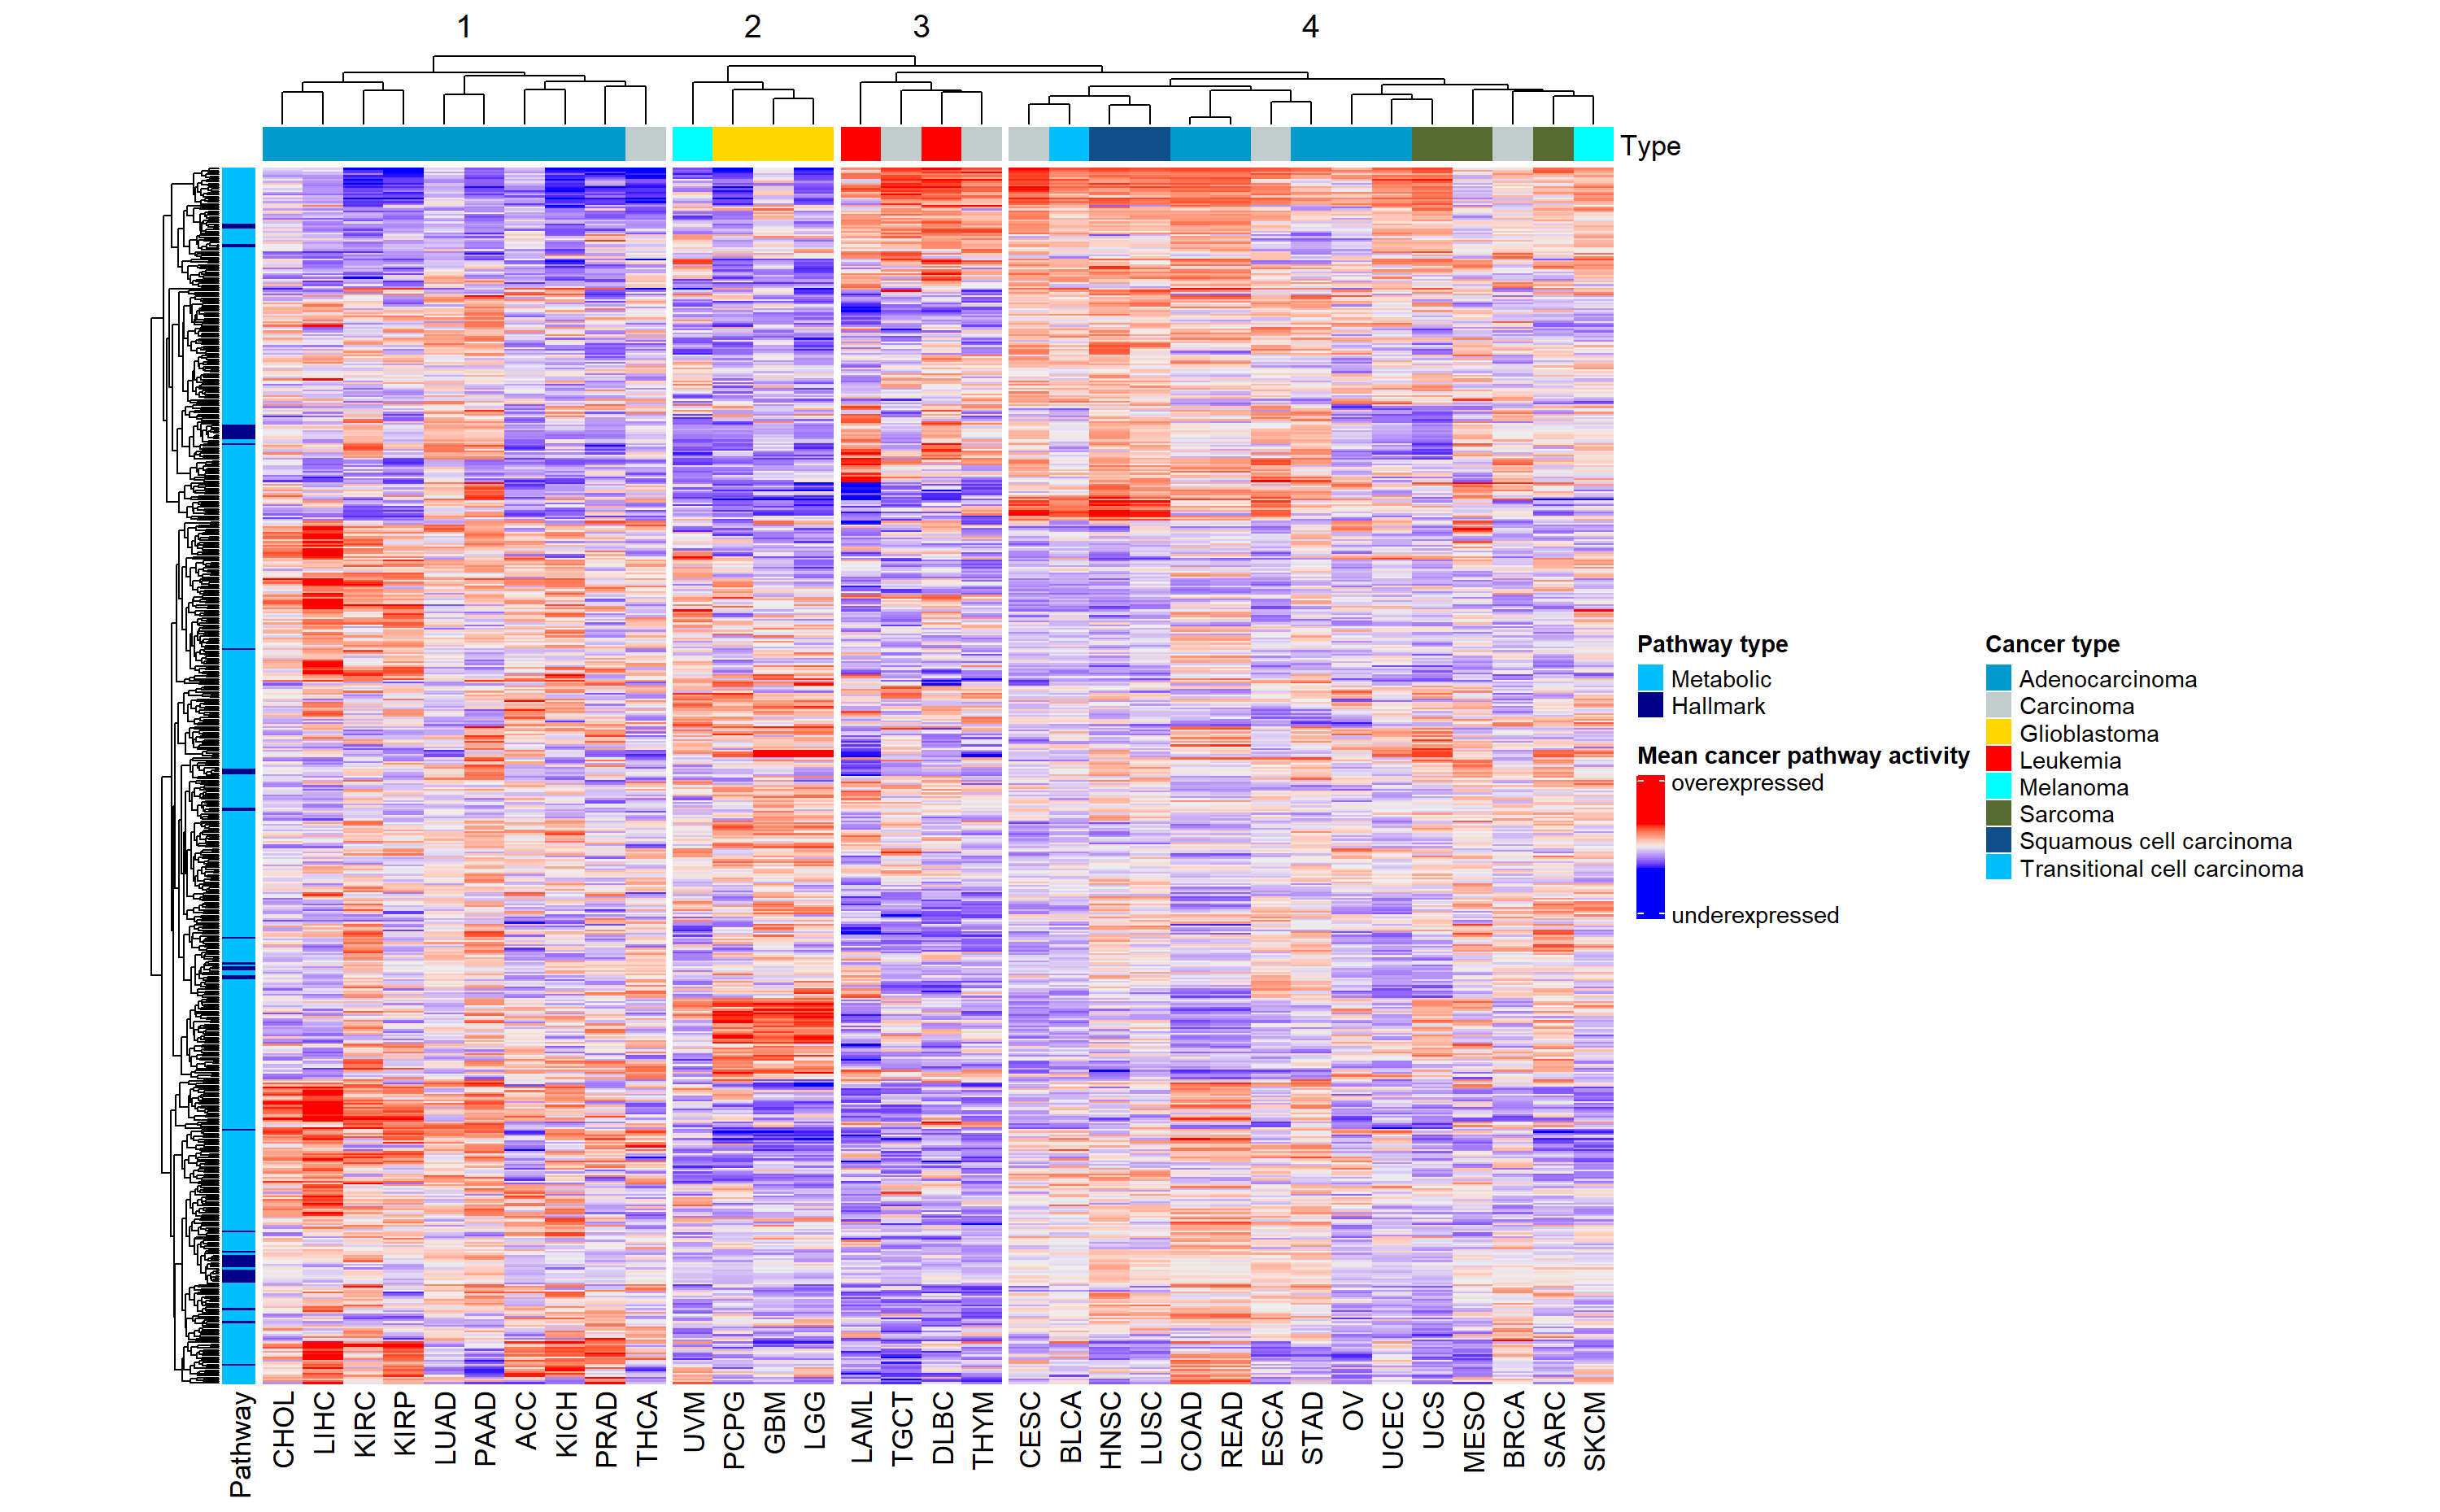
\includegraphics[width=0.5\linewidth]{figures/Pan Cancer mean expression} 

}

\caption{Mean expression of each pathway in each tumot type, annotated with pathway type, histological cancer type and clusters.}\label{fig:meanexp}
\end{figure}

\hypertarget{pca-1}{%
\subsection{PCA}\label{pca-1}}

\hypertarget{dimension-reduction-of-gsva-pan-cancer-data-reveals-clusters-in-pathway-activity}{%
\subsection{Dimension reduction of GSVA pan-cancer data reveals clusters
in pathway
activity}\label{dimension-reduction-of-gsva-pan-cancer-data-reveals-clusters-in-pathway-activity}}

PCA was performed on GSVA pan-cacner data to provide uncorrelted
varibales for better UMAP analysis. No apparent clustering was observed
only in PCA data (compare Figure xxx supplementray materail). Subsequent
UMAP analysis however, showed clear clusters for most cancer types.
@ref(fig:UMAPPanType) @ref(fig:UMAPPanForm). This complemetns the
results obtained from our heatmap and reassures, that the tumor types
have characteristic pathway activities. However, some cancers cluster
better with their histological type rather than tumor type. This was
observed mainly for carcinomas like squamous cell carcinoma and
transitional cell carcinoma, as well as sarcoma, lung adenocarcinoma and
ovarian cancer. These are the same histological types that proofed
difficult to cluster in the mean GSVA of TCGA expression. The UMAP
confirmed the assumption, that the histological type of a tumor has a
major impact on the patients gene expression profile.

\begin{figure}

{\centering 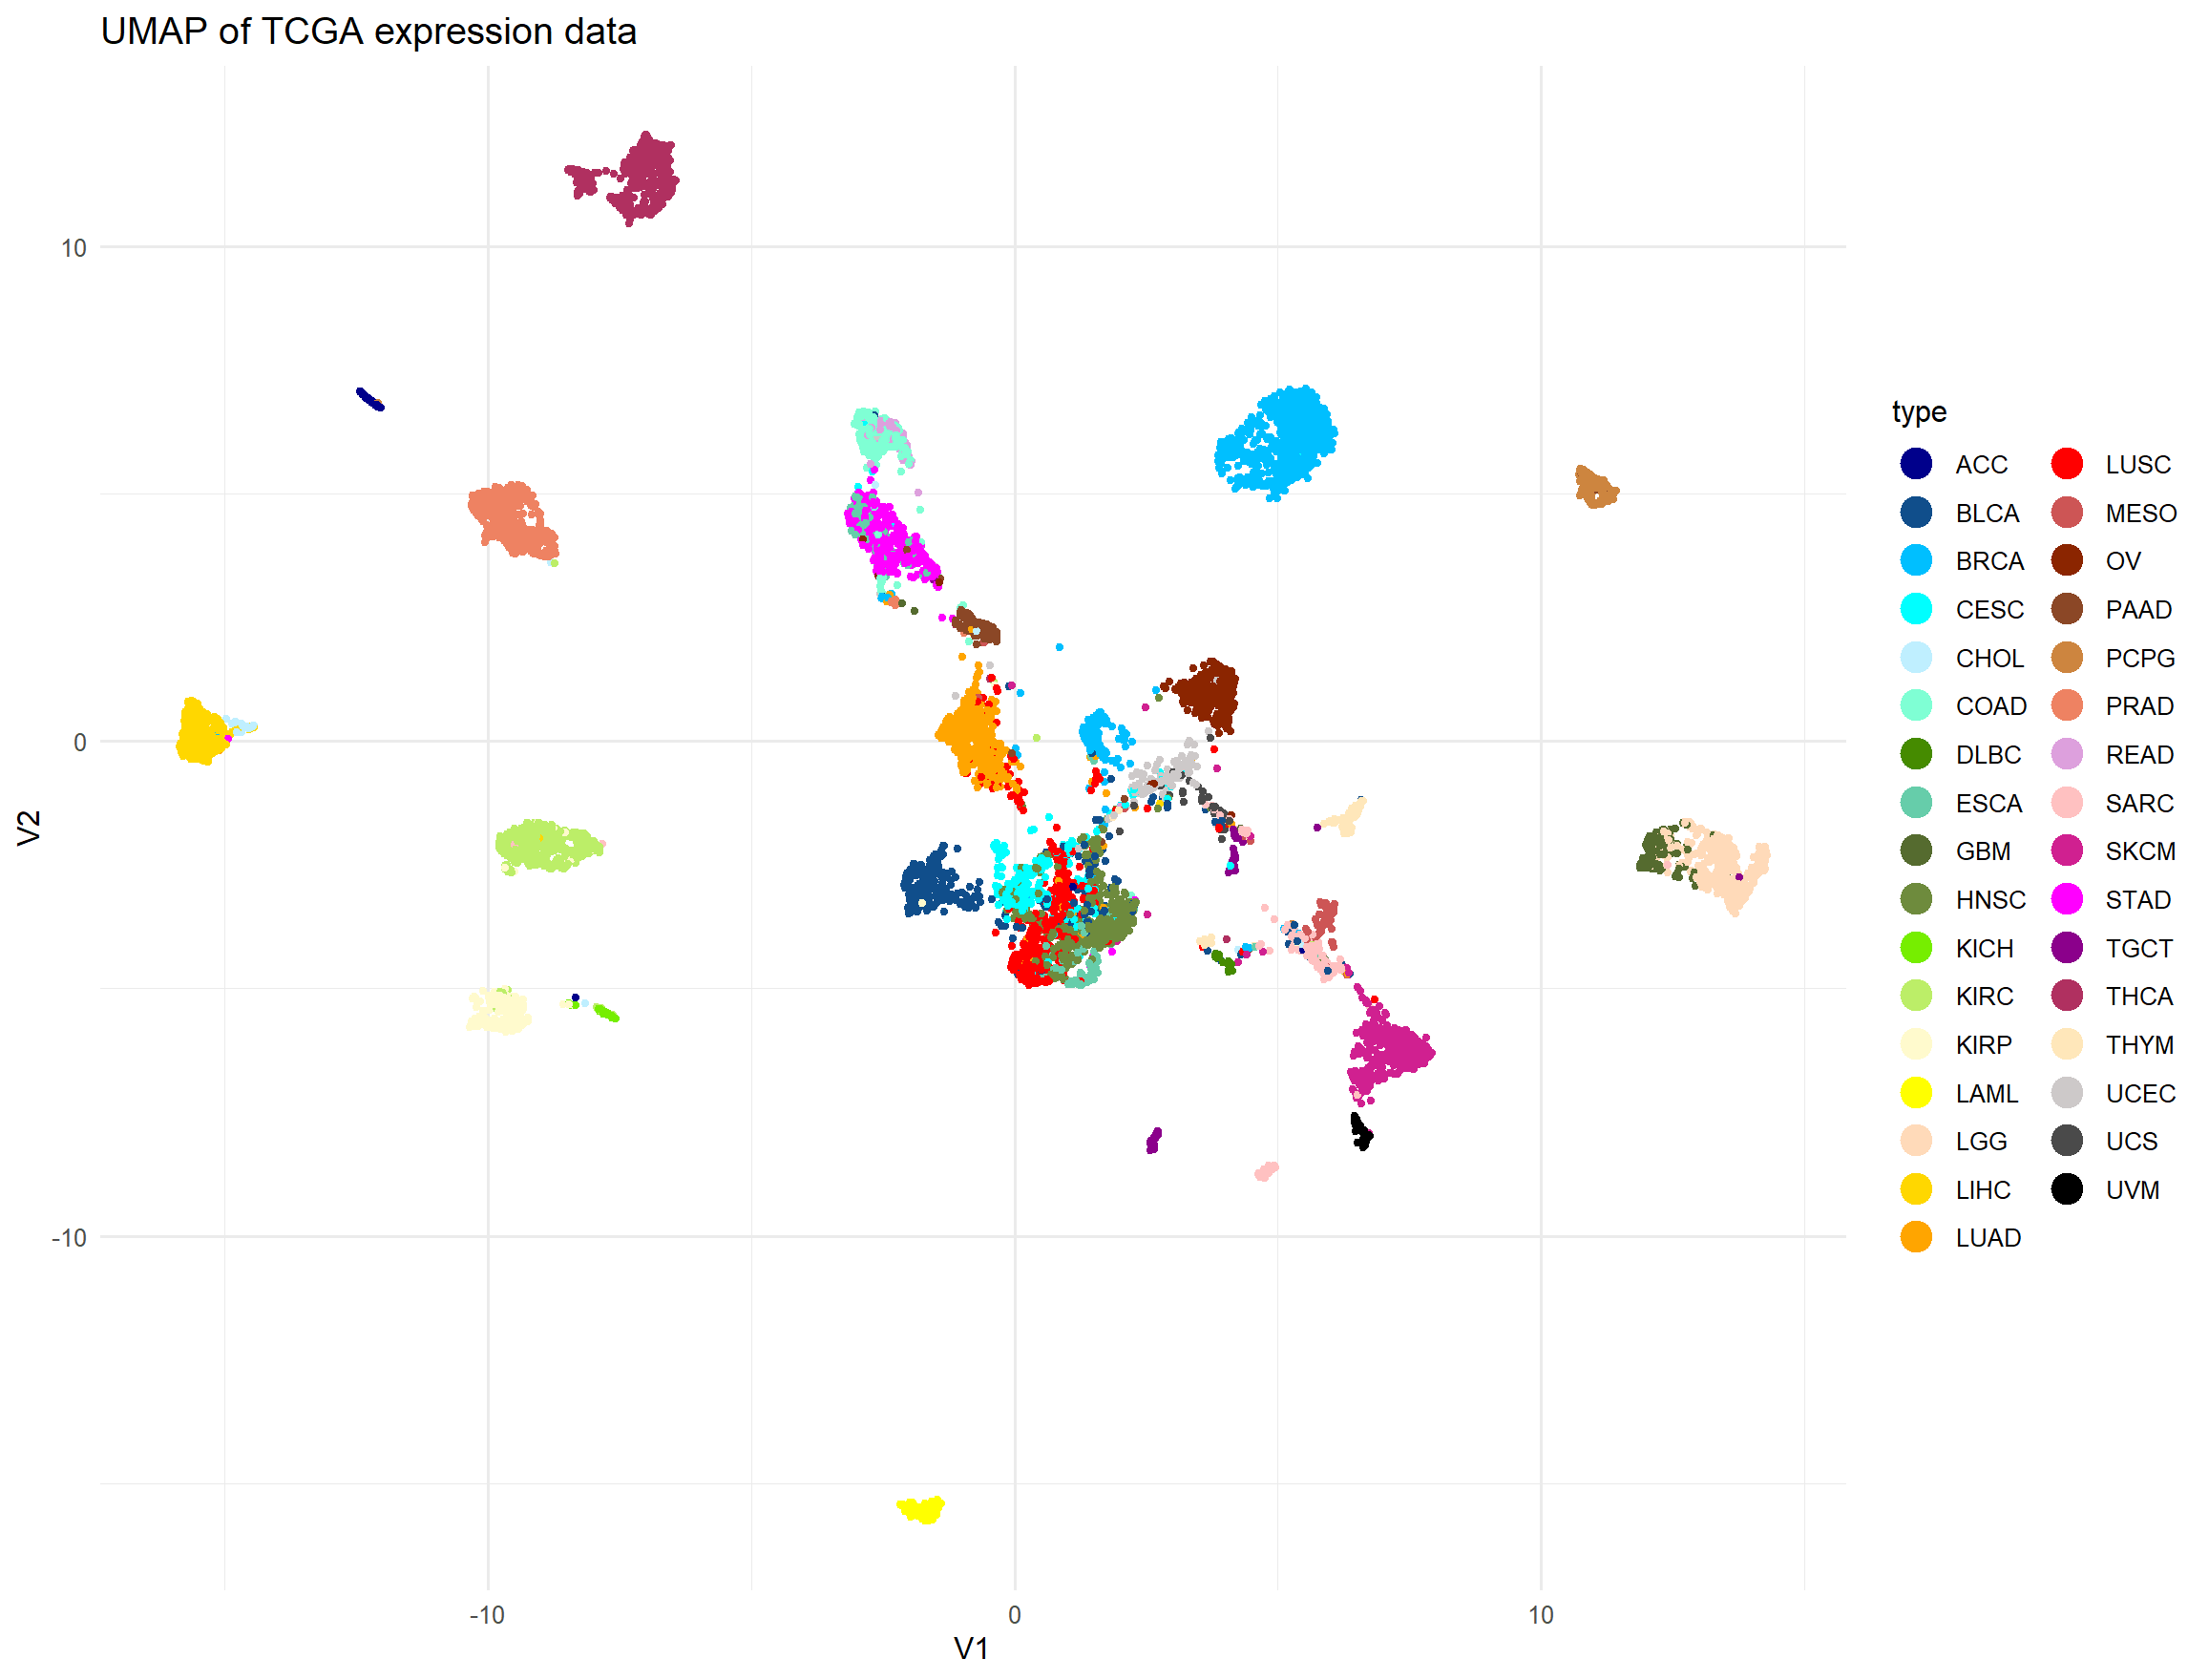
\includegraphics[width=0.5\linewidth]{figures/Pan Cancer UMAP} 

}

\caption{UMAP of TCGA expression data, colored by tumor type}\label{fig:UMAPPanType}
\end{figure}

\begin{figure}

{\centering 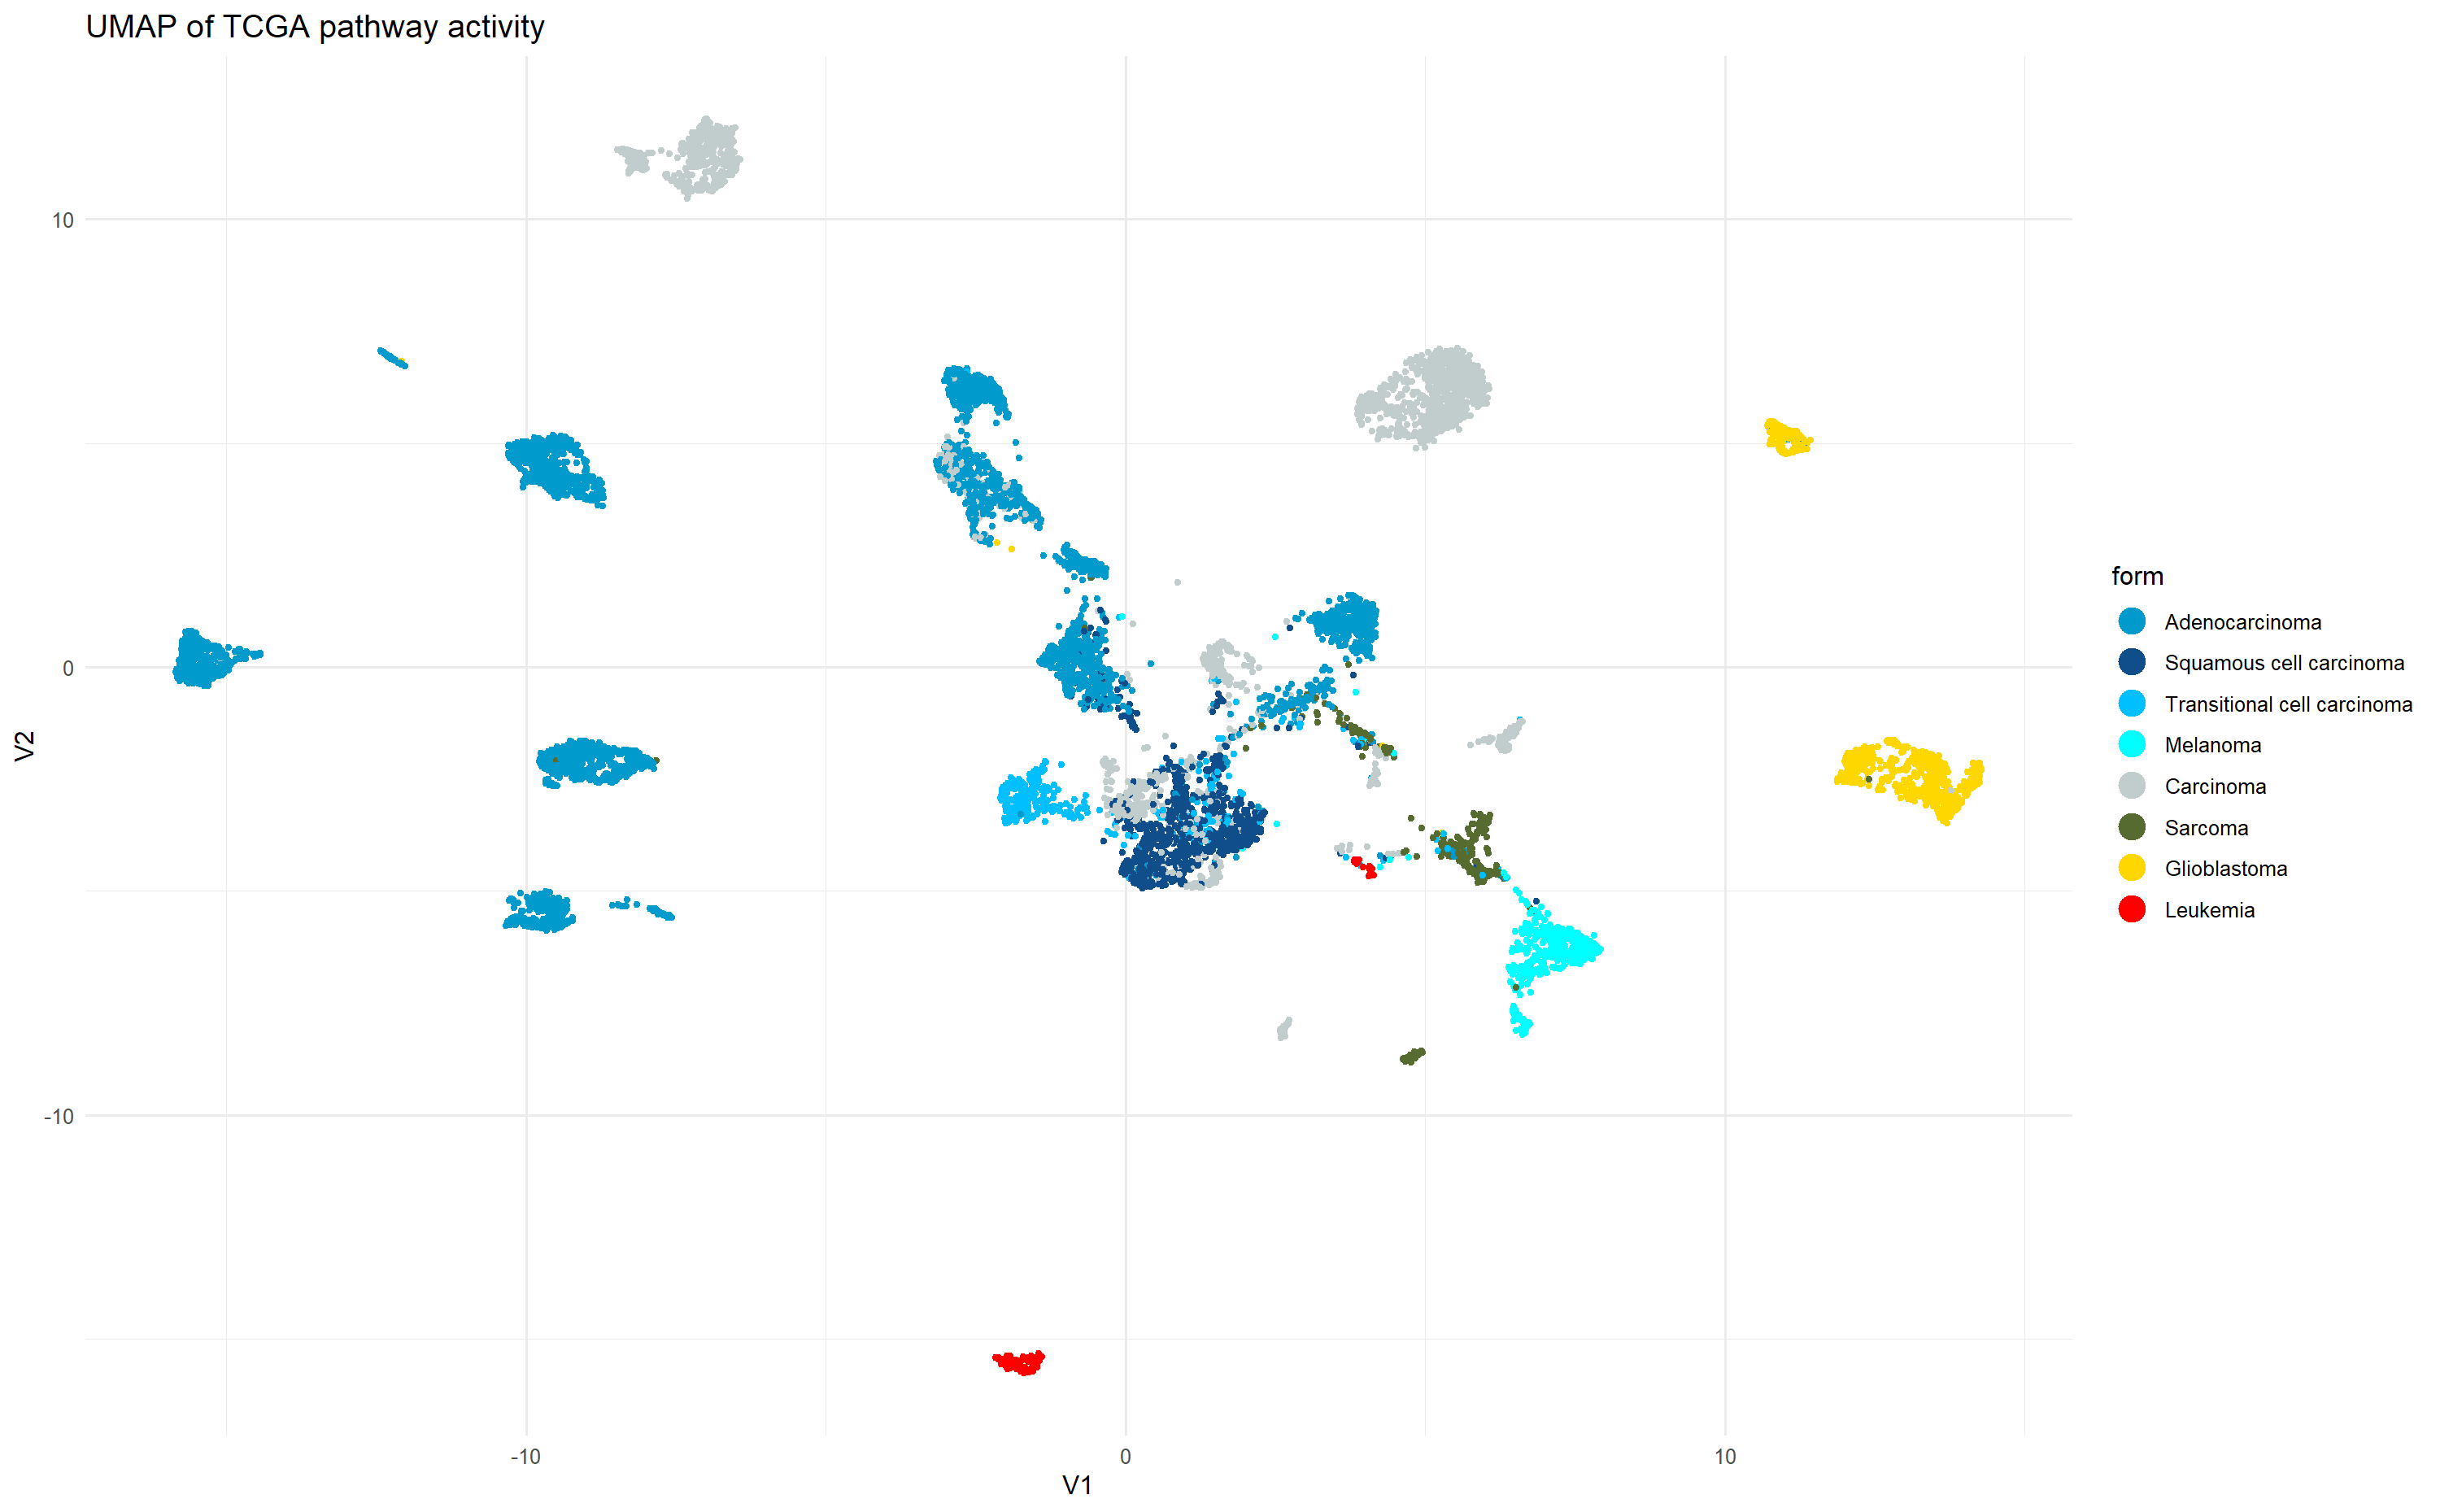
\includegraphics[width=0.5\linewidth]{figures/Pan Cancer UMAP cancer form} 

}

\caption{UMAP of TCGA expression data, colored by form of the tumor}\label{fig:UMAPPanForm}
\end{figure}

The same analysis was performed for gene expression activity instead of
pathway activity to check for reliability of the results. Similar
clusters were observed, which confirms our results (see Fig.
appendix)xxx.

\hypertarget{focused-analysis}{%
\section{Focused analysis}\label{focused-analysis}}

\hypertarget{gsva-on-thca-expression-data-reveals-pathways-driving-thyroid-carcinogenesis.}{%
\subsection{GSVA on THCA expression data reveals pathways driving
thyroid
carcinogenesis.}\label{gsva-on-thca-expression-data-reveals-pathways-driving-thyroid-carcinogenesis.}}

To grasp a general overview of the differences in pathway activity
between THCA and homeostatic thyroid tissue, GSVA was performed for the
THCA expression data. Then, changes in pathway activity were computed by
log2 fold change and the respective p-values were computed by a Wilcoxon
rank-sum test. The most significantly altered pathways were then
characterized. Most prominently among them were pathways linked to
proliferative signaling such as upregulation of p53 inhibitory proteins
and hedgehog pathway activating Gli proteins. Further, the alpha6beta4
integrin signaling pathway and associated pathways such as IL-36
signaling and Typ I hemidesmosome synthesis were significantly enhanced
in THCA. These findings are consistent with previous studies that linked
alpha6beta4 signaling to the development of aggressive forms of thyroid
cancer Noh \emph{et al.} (2010). Also, oncogenic signaling pathways
commonly associated with different cancer types were significantly
upregulated in THCAs. Among them, we observed ERBB2 QUELLE MSigDB and
MST1 signaling commonly found in breast cancer. A role for MSP/Ron in
breast cancer has recently been elucidated, wherein this pathway
regulates tumor growth, angiogenesis, and metastasis (Kretschmann
\emph{et al.}, 2010).

Further, signaling through the EWSR1/FL1-fusion protein was
significantly upregulated in THCA and previously shown to promote the
rapid development of myeloid/erythroid leukemia in mice Quelle Msigdb.
Lastly, THCAs showed downregulation of non-histone protein methylation.
This process was identified as an import modulator of intracellular
signaling by the MAPK, WNT, BMP, Hippo, and JAK/STAT pathways and might
play an important role as a driver of carcinogenesis in THCA (Biggar and
Li, 2015). Together these findings give a general overview of mechanisms
driving carcinogenesis in THCA. However, no information about possible
THCA subtypes or differences in patway activity between patients can be
obtained from this data.

\hypertarget{pan-cancer-data-gsva-reveals-three-subtypes-of-thca-altering-in-proliferative-signaling.}{%
\subsection{Pan-cancer data GSVA reveals three subtypes of THCA altering
in proliferative
signaling.}\label{pan-cancer-data-gsva-reveals-three-subtypes-of-thca-altering-in-proliferative-signaling.}}

To investigate potential subtypes of THCA, the respective samples were
taken from the pan-cancer GSVA data. The optimal number of clusters was
determined by an elbow plot and subsequent K-means clustering revealed a
total of three subtypes in THCA. This is consistent with the three
clusters of THCA observed in the full pan-cancer GSVA data. The
follicular histological type was enriched in cluster B, with no tall
cell types present in this cluster. Judging from histological type alone
no difference in clusters A and C was observed. Most significant changes
in pathway activity were observed in pathways concerning proliferative
signaling. In comparison with all other tumor types, cluster A displayed
high activity of RAS, JAK/STAT and EWSR1/FL1-fusion mediated signaling
as well as elevated signatures associated with carcinogenesis driven by
alpha6beta4 activity. In contrast, these pathways were downregulated in
cluster B, with it showing elevated activity in mTOR, MAPK, PI3K, and
EGFR signaling cascades. Cluster C was found to upregulate all the
aforementioned forms of proliferative signaling. All clusters showed a
homogenous upregulation of hedgehog, ERBB2, and MST1 pathway activity.
Regarding immune response, cluster C showed no significant alterations
in the respective hallmark pathways, however, these pathways were
downregulated in both clusters A and B. With this data, we can identify
two seemingly different forms of proliferative signaling driving
carcinogenesis in THCA. These forms can either occur separately as in
the case of clusters A and B or combined as for cluster C.

\hypertarget{thca-subtypes-do-not-differ-in-their-metabolism.}{%
\subsection{THCA subtypes do not differ in their
metabolism.}\label{thca-subtypes-do-not-differ-in-their-metabolism.}}

To investigate how the identified subtypes compare to homeostatic
thyroid tissue, GSEA was performed for the THCA data. Consistent with
the pan-cancer analysis of THCA data, k-means clustering obtained three
different clusters in pathway activity -- verified as the optimal number
of clusters via an elbow plot. All clusters showed a similar change in
metabolism. Katabolic pathways are downregulated whereas anabolic
pathways e.g., fatty acid synthesis show increased activity in
comparison with normal tissue. These changes in metabolic activity are
in line with the Warburg effect. Further, the results seem consistent
with the proliferative signaling activities found previously.
Alpha6beta4, RAS, JAK/STAT, and EWSR1/FL1-fusion mediated signaling is
upregulated in clusters one and three with low expression in cluster
two. However, the expected upregulation of mTOR, MAPK, PI3K, and EGFR
signaling in clusters two and three was observed only in some samples.
Regarding, immune response the expression profiles are again consistent
with differences observed in the GSVA pan-cancer data: Both clusters one
and two show a lower immune response compared to cluster three. From
these GSEA results, we can conclude that the three subtypes of THCA
differ in carcinogenesis and associated immune response but share a
similar metabolism consistent with the Warburg effect.

\hypertarget{regression-analysis-of-thca-pathway-activity}{%
\section{Regression analysis of THCA pathway
activity}\label{regression-analysis-of-thca-pathway-activity}}

To select a suitable pathway for regression analysis, the top 20\%
pathways regarding their variance in activity were chosen, as for the
regression model to predict. Pathways with little variance were found to
be better predicted by a null model (Fig xxx supplementary material). To
factor in biological significance, the intersect of the 25 most
significantly altered pathways from GSVA with the high variance pathways
was computed. This resulted in three significantly altered and highly
variant pathways among which the REACTOME\_INTERLEUKIN\_36\_PATHWAY gene
set was selected. This gene set ranks 8th among the highest upregulated
pathways with an associated p-value of 8.411155e-15. As interleukin 36
signaling is connected to both MAPK activity and through the activation
of NF-kB also the expression of integrin alpha6beta4 effective
regression might be crucial in finding potentially druggable targets in
combating THCA(Queen \emph{et al.}, 2019) Msigdb xxx. Parathyroid
hormone-related protein regulates integrin α6 and β4 levels via
transcriptional and post-translational pathways Regression of the
REACTOME\_INTERLEUKIN\_36\_PATHWAY gene set showed mixed results.

As expected, the neuronal network performed best on the test data with a
mean squared error (MSE) of 0.06. However, the linear regression model
failed to predict the data accurately (MSE = 0.62). Repeated linear
regression with just pathways contributing significantly to the result
the performance was enhanced (MSE = 0.40), however, remained worse than
a null model (MSE = 0.22). (Fig. xxx) A comparison of the four
regression models via the F-test function \texttt{\{var.test()\}} showed
a significant improvement of the neuronal network compared to all other
models. All other models showed no significant differences in their
performance (Fig. xxx) compared to each other. From this data, we can
conclude that a neuronal network is the best choice for most accurately
predicting IL-36 pathway activity in our test data.

\begin{center}\rule{0.5\linewidth}{0.5pt}\end{center}

\hypertarget{discussion}{%
\chapter{Discussion}\label{discussion}}

In der PCA war nicht so ein gutes Ergebnis zu erkennen, weil nur die
ersten 2 PCs verwendet wurden und dadurch nicht die gesamte Varianz
erklärt wurde, durch die Verwendung von mehr PCs oder von anderen PCs
(zB 2 und 3) könnte man evtl. eine bessere Darstellung erhalten. Bei
verwendung aller PCs in der UMAP waren eindeutige Cluster zu erkennen
allerdings ist UMAP auch nicht die optimale Methode, weil da die
Abstände innerhalb der Cluster nicht proportional zu den tatsächlichen
Abständen sind weil die mehrdimensionalen Daten irgendwie auf 2
Dimensionen runtergebrochen werden mussten.

Die Ergebnisse der UMAPs entsprechen der Erwartungen. Carcinomas haben
alle ähnliche Expressionsmuster, da sie alle epithelialen Zellen
entspringen und deshalb ähnliche genetische Mechanismen brauchen, um zu
einer Tumorzelle zu werden. Die expressionsmuster zu anderen
histological tumor types unterscheiden sich. Das liegt daran, dass
verschiedene genetische Mechanismen zur Tumorentstehung führen, da sie
anderen Zellen entspringen. Dadurch ist auch die unterschiedliche
Genexpression zwischen den einzelnen Tumortypen, die zwar den gleichen
histological type haben, aber sich in ihrem Tumortyp unterscheiden, wie
zB die Adenocarcionma.

Die Ergebnisse der GSVA \ldots{}

GSVA mittlerer expressionswerte: dass hallmark pathways alle weiß sind
entspricht unseren erwartungen

Outlook:

Epigeentic profiles = auch epigenetische veränderungen werden in die
Expressionsdate mit inebezogen, das wäre sehr sinnvol für die ANalyse,
wird hier aber nicht beachetet

Vergleich zwischen GSVA und GSEA --\textgreater{} weil einmal Vergleich
mit tumor und normal

\hypertarget{references}{%
\chapter{References}\label{references}}

\hypertarget{refs}{}
\begin{CSLReferences}{0}{0}
\leavevmode\vadjust pre{\hypertarget{ref-cell}{}}%
Alberts, J, B., and Walter, P (2015). Molecular biology of the cell, New
York: Garland science.

\leavevmode\vadjust pre{\hypertarget{ref-result5}{}}%
Ben-Porath, I, Thomson, MW, Carey, VJ, Ge, R, Bell, GW, Regev, A, and
Weinberg, RA (2008). An embryonic stem cell-like gene expression
signature in poorly differentiated aggressive human tumors. Nat Genet
40, 499--507.

\leavevmode\vadjust pre{\hypertarget{ref-result1}{}}%
Biggar, KK, and Li, SSC (2015). Non-histone protein methylation as a
regulator of cellular signalling and function. Nature Reviews Molecular
Cell Biology 16, 5--17.

\leavevmode\vadjust pre{\hypertarget{ref-THCA}{}}%
Cabanillas, ME, McFadden, DG, and Durante, C (2016). Thyroid cancer.
Lancet 388, 2783--2795.

\leavevmode\vadjust pre{\hypertarget{ref-PCA_aggressive}{}}%
Coca-Pelaz, A et al. (2020). Papillary thyroid cancer-aggressive
variants and impact on management: A narrative review. Adv Ther 37,
3112--3128.

\leavevmode\vadjust pre{\hypertarget{ref-biomaRt}{}}%
Durinck, S, Moreau, Y, Kasprzyk, A, Davis, S, De Moor, B, Brazma, A, and
Huber, W (2005). BioMart and bioconductor: A powerful link between
biological databases and microarray data analysis. Bioinformatics 21,
3439--3440.

\leavevmode\vadjust pre{\hypertarget{ref-cancer_hallmarks}{}}%
Hanahan, D, and Weinberg, RA (2011). Hallmarks of cancer: The next
generation. Cell 144, 646--674.

\leavevmode\vadjust pre{\hypertarget{ref-GSVA}{}}%
Hänzelmann, S, Castelo, R, and Guinney, J (2013). GSVA: Gene set
variation analysis for microarray and RNA-seq data. BMC Bioinformatics
14, 7.

\leavevmode\vadjust pre{\hypertarget{ref-PCA3}{}}%
Kant, R, Davis, A, and Verma, V (2020). Thyroid nodules: Advances in
evaluation and management. Am Fam Physician 102, 298--304.

\leavevmode\vadjust pre{\hypertarget{ref-result2}{}}%
Kretschmann, KL, Eyob, H, Buys, SS, and Welm, AL (2010). The macrophage
stimulating protein/ron pathway as a potential therapeutic target to
impede multiple mechanisms involved in breast cancer progression. Curr
Drug Targets 11, 1157--1168.

\leavevmode\vadjust pre{\hypertarget{ref-PCA1}{}}%
Lin, JD (2007). Papillary thyroid carcinoma with lymph node metastases.
Growth Factors 25, 41--49.

\leavevmode\vadjust pre{\hypertarget{ref-result3}{}}%
Noh, TW, Soung, YH, Kim, HI, Gil, HJ, Kim, JM, Lee, EJ, and Chung, J
(2010). Effect of {beta}4 integrin knockdown by RNA interference in
anaplastic thyroid carcinoma. Anticancer Res 30, 4485--4492.

\leavevmode\vadjust pre{\hypertarget{ref-THCA2}{}}%
Prete, A, Borges de Souza, P, Censi, S, Muzza, M, Nucci, N, and
Sponziello, M (2020). Update on fundamental mechanisms of thyroid
cancer. Front Endocrinol (Lausanne) 11, 102.

\leavevmode\vadjust pre{\hypertarget{ref-result4}{}}%
Queen, D, Ediriweera, C, and Liu, L (2019). Function and regulation of
IL-36 signaling in inflammatory diseases and cancer development. Front
Cell Dev Biol 7, 317.

\leavevmode\vadjust pre{\hypertarget{ref-GSEA}{}}%
Reimand, J et al. (2019). Pathway enrichment analysis and visualization
of omics data using g:profiler, GSEA, cytoscape and EnrichmentMap.
Nature Protocols 14, 482--517.

\leavevmode\vadjust pre{\hypertarget{ref-UMAP}{}}%
Sharma, S, Quinn, D, Melenhorst, JJ, and Pruteanu-Malinici, I (2021).
High-dimensional immune monitoring for chimeric antigen receptor t cell
therapies. Current Hematologic Malignancy Reports 16, 112--116.

\leavevmode\vadjust pre{\hypertarget{ref-THgland1}{}}%
Tsibulnikov, S, Maslov, L, Voronkov, N, and Oeltgen, P (2020). Thyroid
hormones and the mechanisms of adaptation to cold. Hormones (Athens) 19,
329--339.

\leavevmode\vadjust pre{\hypertarget{ref-result6}{}}%
Wang, X, Pei, Z, Hossain, A, Bai, Y, and Chen, G (2021). Transcription
factor-based gene therapy to treat glioblastoma through direct neuronal
conversion. Cancer Biol Med 18, 860--874.

\end{CSLReferences}

\hypertarget{appendix}{%
\chapter{Appendix}\label{appendix}}

\hypertarget{plots}{%
\section{Plots}\label{plots}}

\begin{figure}

{\centering 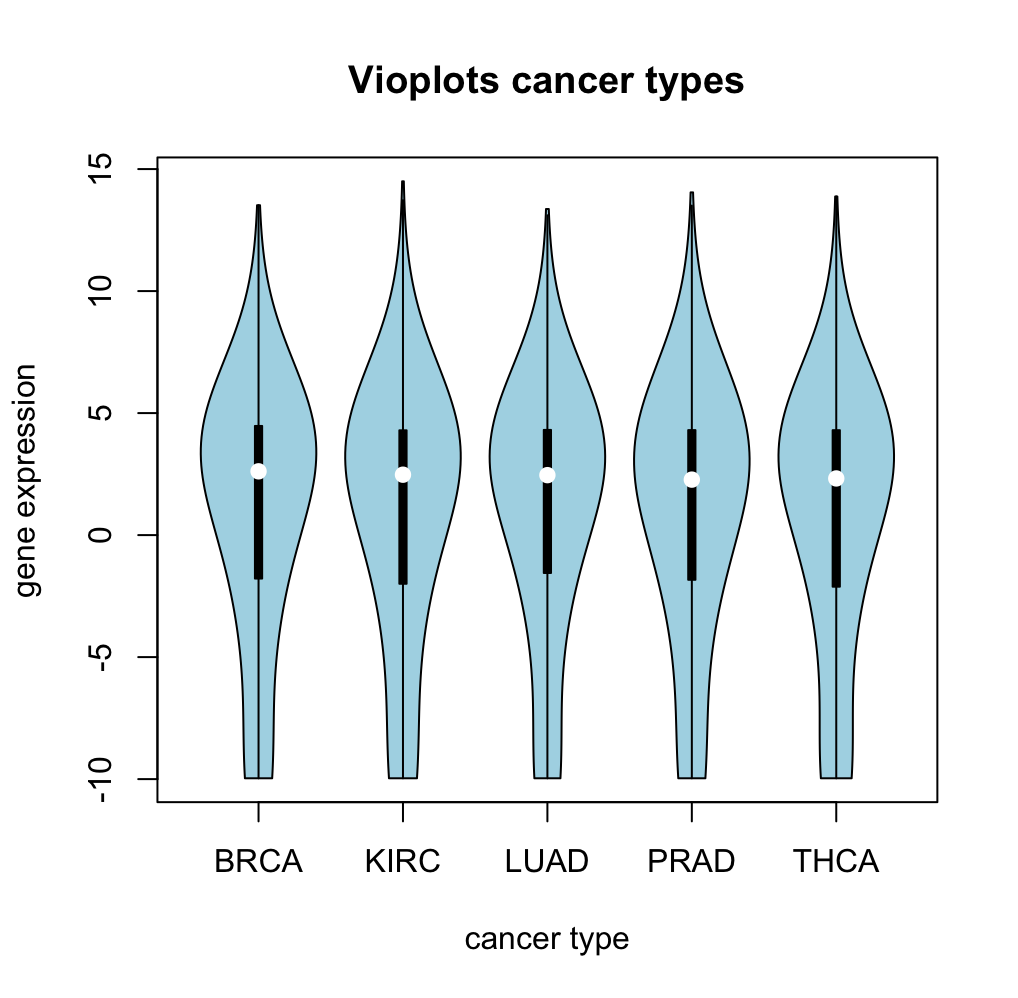
\includegraphics[width=0.3\linewidth]{figures/Vioplots cancer types} 

}

\caption{Mean-variance plot of cleaned TCGA expression data}\label{fig:showviolinplots}
\end{figure}

\hypertarget{code}{%
\section{Code}\label{code}}

world

\begin{Shaded}
\begin{Highlighting}[]
\CommentTok{\#createn einer liste mit allen patienten in dfs sortiert nach krebs}
\NormalTok{cancers }\OtherTok{=} \FunctionTok{list}\NormalTok{();cancers }\OtherTok{=} \FunctionTok{vector}\NormalTok{(}\StringTok{\textquotesingle{}list\textquotesingle{}}\NormalTok{,}\FunctionTok{length}\NormalTok{(}\FunctionTok{table}\NormalTok{(tcga\_anno}\SpecialCharTok{$}\NormalTok{cancer\_type\_abbreviation)))}
\FunctionTok{names}\NormalTok{(cancers) }\OtherTok{=} \FunctionTok{names}\NormalTok{(}\FunctionTok{table}\NormalTok{(tcga\_anno}\SpecialCharTok{$}\NormalTok{cancer\_type\_abbreviation))}
\NormalTok{i}\OtherTok{=}\DecValTok{1}
\ControlFlowTok{for}\NormalTok{ (i }\ControlFlowTok{in} \DecValTok{1}\SpecialCharTok{:}\FunctionTok{length}\NormalTok{(cancers))\{}
\NormalTok{  cancers[[i]] }\OtherTok{=}\NormalTok{ tcga\_exp\_cleaned[,tcga\_anno}\SpecialCharTok{$}\NormalTok{cancer\_type\_abbreviation }\SpecialCharTok{==} \FunctionTok{names}\NormalTok{(cancers)[i]]}
\NormalTok{\}}
\CommentTok{\#function die einen krebstypen df und genesets als input nimmt und ein df mit pvalues ausgibt}
\NormalTok{enrichment }\OtherTok{=} \ControlFlowTok{function}\NormalTok{(expressiondata, }\AttributeTok{genesets =}\NormalTok{ genesets\_ids)\{}
\NormalTok{  ESmatrix }\OtherTok{=} \FunctionTok{sapply}\NormalTok{(genesets, }\AttributeTok{FUN =} \ControlFlowTok{function}\NormalTok{(x)\{}
\NormalTok{    ins }\OtherTok{=} \FunctionTok{na.omit}\NormalTok{(}\FunctionTok{match}\NormalTok{(x,}\FunctionTok{rownames}\NormalTok{(expressiondata)))}\CommentTok{\#indices der gene im aktuellen set}
\NormalTok{    outs }\OtherTok{=} \SpecialCharTok{{-}}\NormalTok{ins}\CommentTok{\#indices der gene nicht im aktuellen set}
    \CommentTok{\#gibt einen vektor der für jeden patienten den pval für das aktuelle gene enthält}
\NormalTok{    res }\OtherTok{=} \ConstantTok{NULL}
    \ControlFlowTok{for}\NormalTok{ (i }\ControlFlowTok{in} \DecValTok{1}\SpecialCharTok{:}\FunctionTok{ncol}\NormalTok{(expressiondata))\{}\CommentTok{\#testet für jeden patienten}
\NormalTok{      res[i] }\OtherTok{=} \FunctionTok{wilcox.test}\NormalTok{(expressiondata[ins,i],expressiondata[outs,i],}\StringTok{\textquotesingle{}two.sided\textquotesingle{}}\NormalTok{)}\SpecialCharTok{$}\NormalTok{p.value}
\NormalTok{    \}}
    \FunctionTok{return}\NormalTok{(res)}
\NormalTok{  \})}
  \FunctionTok{row.names}\NormalTok{(ESmatrix) }\OtherTok{=} \FunctionTok{colnames}\NormalTok{(expressiondata); }\FunctionTok{return}\NormalTok{(ESmatrix)}
\NormalTok{\}}
\NormalTok{pvalueslist }\OtherTok{=} \FunctionTok{lapply}\NormalTok{(cancers, enrichment)}\CommentTok{\#für die tests für jeden krebstypen durch}
\end{Highlighting}
\end{Shaded}

\begin{Shaded}
\begin{Highlighting}[]
\NormalTok{get\_top10pathways\_from\_pvalues }\OtherTok{=} \ControlFlowTok{function}\NormalTok{(df\_p\_values, length\_genesets) \{}
  
  \FunctionTok{require}\NormalTok{(ggplot2)}
  
\NormalTok{  results }\OtherTok{\textless{}{-}} \FunctionTok{list}\NormalTok{()}
    
\NormalTok{  df\_p\_values\_log10 }\OtherTok{\textless{}{-}} \SpecialCharTok{{-}}\FunctionTok{log10}\NormalTok{(}\FunctionTok{as.data.frame}\NormalTok{(df\_p\_values))}
    
\NormalTok{  mean\_pathway }\OtherTok{\textless{}{-}} \FunctionTok{as.data.frame}\NormalTok{(}\FunctionTok{apply}\NormalTok{(df\_p\_values\_log10, }\DecValTok{1}\NormalTok{, mean))}
  \FunctionTok{rownames}\NormalTok{(mean\_pathway) }\OtherTok{\textless{}{-}} \FunctionTok{rownames}\NormalTok{(df\_p\_values\_log10)}
  
\NormalTok{  ordered\_score }\OtherTok{\textless{}{-}}\NormalTok{ mean\_pathway[}\FunctionTok{order}\NormalTok{(}\SpecialCharTok{{-}}\NormalTok{mean\_pathway[ ,}\DecValTok{1}\NormalTok{]), }\DecValTok{1}\NormalTok{]}
\NormalTok{  top\_10 }\OtherTok{\textless{}{-}} \FunctionTok{data.frame}\NormalTok{(ordered\_score[}\DecValTok{1}\SpecialCharTok{:}\DecValTok{10}\NormalTok{])}
  \FunctionTok{colnames}\NormalTok{(top\_10) }\OtherTok{\textless{}{-}} \StringTok{"mean\_pathway"}
  
\NormalTok{  ordered\_names }\OtherTok{\textless{}{-}} \FunctionTok{order}\NormalTok{(}\SpecialCharTok{{-}}\NormalTok{mean\_pathway[ ,}\DecValTok{1}\NormalTok{])}
\NormalTok{  top\_10\_names }\OtherTok{\textless{}{-}}\NormalTok{ ordered\_names[}\DecValTok{1}\SpecialCharTok{:}\DecValTok{10}\NormalTok{]}
\NormalTok{  top\_10}\SpecialCharTok{$}\NormalTok{pathway\_names }\OtherTok{\textless{}{-}} \FunctionTok{row.names}\NormalTok{(mean\_pathway)[top\_10\_names]}
  
\NormalTok{  results[[}\DecValTok{1}\NormalTok{]] }\OtherTok{\textless{}{-}}\NormalTok{ top\_10}
  
\NormalTok{  results[[}\DecValTok{2}\NormalTok{]] }\OtherTok{\textless{}{-}} \FunctionTok{ggplot}\NormalTok{(}\AttributeTok{data =}\NormalTok{ top\_10, }\FunctionTok{aes}\NormalTok{(}\AttributeTok{x =}\NormalTok{ mean\_pathway, }\AttributeTok{y =} \FunctionTok{reorder}\NormalTok{(pathway\_names, mean\_pathway)))}\SpecialCharTok{+}
    \FunctionTok{geom\_bar}\NormalTok{(}\AttributeTok{stat =} \StringTok{"identity"}\NormalTok{)}\SpecialCharTok{+}
    \FunctionTok{coord\_cartesian}\NormalTok{(}\AttributeTok{xlim =}\FunctionTok{c}\NormalTok{(}\DecValTok{3}\NormalTok{, }\FloatTok{3.75}\NormalTok{))}\SpecialCharTok{+}
    \FunctionTok{labs}\NormalTok{(}\AttributeTok{title =} \FunctionTok{names}\NormalTok{(df\_p\_values),}
         \AttributeTok{x =} \StringTok{"mean p{-}value pathway"}\NormalTok{,}
         \AttributeTok{y =} \StringTok{"pathway name"}\NormalTok{)}
  
\NormalTok{  pathway\_size }\OtherTok{\textless{}{-}} \FunctionTok{order}\NormalTok{(}\SpecialCharTok{{-}}\NormalTok{mean\_pathway[ ,}\DecValTok{1}\NormalTok{])}
\NormalTok{  top\_10\_size }\OtherTok{\textless{}{-}}\NormalTok{ pathway\_size[}\DecValTok{1}\SpecialCharTok{:}\DecValTok{10}\NormalTok{]}
\NormalTok{  top\_10}\SpecialCharTok{$}\NormalTok{pathway\_size }\OtherTok{\textless{}{-}}\NormalTok{ length\_genesets[top\_10\_size]}
  
\NormalTok{  results[[}\DecValTok{3}\NormalTok{]] }\OtherTok{\textless{}{-}} \FunctionTok{ggplot}\NormalTok{(}\AttributeTok{data =}\NormalTok{ top\_10, }\FunctionTok{aes}\NormalTok{(}\AttributeTok{x =}\NormalTok{ mean\_pathway, }\AttributeTok{y =} \FunctionTok{reorder}\NormalTok{(pathway\_names,}
\NormalTok{                                                                          mean\_pathway)))}\SpecialCharTok{+}
    \FunctionTok{geom\_point}\NormalTok{(}\FunctionTok{aes}\NormalTok{(}\AttributeTok{size =}\NormalTok{ pathway\_size))}\SpecialCharTok{+}
    \FunctionTok{labs}\NormalTok{(}\AttributeTok{title =} \FunctionTok{names}\NormalTok{(df\_p\_values),}
         \AttributeTok{x =} \StringTok{"mean p{-}value pathway"}\NormalTok{,}
         \AttributeTok{y =} \StringTok{"pathway name"}\NormalTok{)}
  
  \FunctionTok{return}\NormalTok{(results)}
\NormalTok{\}}
\end{Highlighting}
\end{Shaded}


\end{document}
